\documentclass[12pt]{amsart}

\usepackage{amsmath,amsfonts,amssymb,mathabx,shuffle,latexsym,breqn,stmaryrd,mathtools,mathrsfs}
\usepackage{enumitem}
\usepackage{subcaption}
\usepackage[usenames, dvipsnames]{xcolor}
\usepackage[backref=page]{hyperref}
\usepackage{ytableau}
\usepackage{tikz-cd}
\usepackage{array}
\usepackage{tikz}
\usetikzlibrary{calc, shapes, backgrounds,arrows.meta,positioning,plotmarks,decorations.markings}
\tikzset{>=Straight Barb,
  head/.style = {fill = white, text=black},
  plaque/.style = {draw, rectangle, minimum size = 10mm}, 
  pil/.style={->,thick},
  pilpil/.style={<->,thick},
  junct/.style = {draw,circle,inner sep=0.5pt,outer sep=0pt, fill=black}
  }
 
%\usepackage{fullpage}
\setlength{\evensidemargin}{0in} 
\setlength{\textheight}{8.4in}      
\setlength{\textwidth}{6in}    
\setlength{\topmargin}{0in}      
\setlength{\oddsidemargin}{0in} 

%%%%%%%%%%%%%%%%%%%%%%%%%%%%%
% Dynkin things
\newcommand{\dynkinradius}{.15cm}
\newcommand{\dynkinstep}{.58cm}
\newcommand{\dynkinnormal}[2]{\fill (\dynkinstep*#1,\dynkinstep*#2) circle (\dynkinradius);}
%\newcommand{\dynkinXsize}{1.5}
\newcommand{\dynkinmin}[2]{\filldraw[fill=SkyBlue,draw=black] (\dynkinstep*#1,\dynkinstep*#2) circle (\dynkinradius);}
\newcommand{\dynkinline}[4]{\draw[thin] (\dynkinstep*#1,\dynkinstep*#2) -- (\dynkinstep*#3,\dynkinstep*#4);}
\newcommand{\dynkindots}[4]{\draw[dotted,very thick] (\dynkinstep*#1,\dynkinstep*#2) -- (\dynkinstep*#3,\dynkinstep*#4);}
\newcommand{\dynkindoubleline}[4]{\draw[double,double distance between line centers=0.19em,postaction={decorate}] (\dynkinstep*#1,\dynkinstep*#2) -- (\dynkinstep*#3,\dynkinstep*#4);}

\newenvironment{dynkin}{\begin{tikzpicture}[decoration={markings,mark=at position 0.7 with {\arrow{>[scale=.7]}}}]}
{\end{tikzpicture}}

\usepackage{enumitem}
\newlist{arrowlist}{itemize}{1}
\setlist[arrowlist]{label=$\Rightarrow$}
\newcommand{\x}{\ensuremath{\mathsf{x}}}
\newcommand{\y}{\ensuremath{\mathsf{y}}}
\newcommand{\e}{\ensuremath{\mathsf{e}}}
\newcommand{\aaa}{\ensuremath{\mathsf{a}}}

\newcommand{\gap}{\hspace{1in} \\ \vspace{-.2in}}


%%%%%%%%%%%%%%%%%%%%%%%%%%%%%%%%%%%%%%%%%%%%%%%%%%%%%%%%%%%%
%  Environments 
%%%%%%%%%%%%%%%%%%%%%%%%%%%%%%%%%%%%%%%%%%%%%%%%%%%%%%%%%%%%

\newtheorem{theorem}{Theorem}[section]
\newtheorem{lemma}[theorem]{Lemma}
\newtheorem{proposition}[theorem]{Proposition}
\newtheorem{corollary}[theorem]{Corollary}
\newtheorem{conjecture}[theorem]{Conjecture}

\theoremstyle{definition}
\newtheorem{definition}[theorem]{Definition}
\newtheorem{examplex}[theorem]{Example}
\newenvironment{example}
  {\pushQED{\qed}\renewcommand{\qedsymbol}{$\diamondsuit$}\examplex}
  {\popQED\endexamplex}
\newtheorem{xca}[theorem]{Exercise}
\newtheorem{algorithm}[theorem]{Algorithm}

\theoremstyle{remark}
\newtheorem{remark}[theorem]{Remark}

\numberwithin{equation}{section}


%%%%%%%%%%%%%%%%%%%%%%%%%%%%%%%%%%%%%%%%%%%%%%%%%%%%%%%%%%%%
%  MACROS for this particular document
%%%%%%%%%%%%%%%%%%%%%%%%%%%%%%%%%%%%%%%%%%%%%%%%%%%%%%%%%%%%

\DeclareMathOperator{\codim}{codim}
\DeclareMathOperator{\ex}{ex}
\newcommand{\wt}{\ensuremath{\mathrm{wt}}}
\newcommand{\rev}{\ensuremath{\mathrm{rev}}}
\newcommand{\inv}{\ensuremath{\mathrm{inv}}}
\newcommand{\reduct}{\ensuremath{\mathtt{reduct}}}
\newcommand{\Des}{\ensuremath{\mathrm{Des}}}
\newcommand{\SSYT}{\ensuremath{\mathrm{SSYT}}}
\newcommand{\SYT}{\ensuremath{\mathrm{SYT}}}
\newcommand{\sit}{\ensuremath{\mathrm{sit}}}
\newcommand{\gen}{\ensuremath{\mathrm{gen}}}
\renewcommand{\emptyset}{\varnothing}

\newcommand{\inc}{\ensuremath{\mathrm{Inc}}}
\newcommand{\incgl}{\inc_{\mathrm{gl}}}
\newcommand{\pro}{\mathfrak{pro}}
\newcommand{\evac}{\mathfrak{Evac}}
\newcommand{\rot}{\ensuremath{\mathsf{rot}}}
\newcommand{\rect}{\ensuremath{\mathsf{rect}}}
\newcommand{\swap}{\ensuremath{\mathsf{swap}}}
\newcommand{\decr}{\ensuremath{\mathsf{Decr}}}
\newcommand{\slide}{\ensuremath{\mathsf{slide}}}
\newcommand{\rep}{\ensuremath{\mathsf{Rep}}}
\newcommand{\blank}{\phantom{2}}
\newcommand{\shape}{\ensuremath{\mathsf{sh}}}
\newcommand{\id}{\ensuremath{\mathrm{id}}}
\newcommand{\bbb}{\ensuremath{\mathsf{b}}}
\newcommand{\rank}{\ensuremath{\mathrm{rk}}}
\newcommand{\mot}{\ensuremath{\mathsf{Mot}}}
\newcommand{\pp}{\ensuremath{\mathsf{PP}}}
\newcommand{\deflate}{\ensuremath{\mathsf{Defl}}}
\newcommand{\inflate}{\ensuremath{\mathsf{VecInfl}}}
\newcommand{\reinflate}{\ensuremath{\mathsf{Reinfl}}}
\newcommand{\tinflate}{\ensuremath{\mathsf{Infl}}}
\newcommand{\content}{\ensuremath{\mathsf{Con}}}
\newcommand{\compress}{\ensuremath{\mathsf{DeflCon}}}

\newcommand{\uu}{\mathcal{I}}

% Fancy comments
\usepackage[colorinlistoftodos]{todonotes}
\newcommand{\holly}[1]{\todo[size=\tiny,color=blue!30]{#1 \\ \hfill --- Holly}}
\newcommand{\Holly}[1]{\todo[size=\tiny,inline,color=blue!30]{#1
      \\ \hfill --- Holly}}
\newcommand{\oliver}[1]{\todo[size=\tiny,color=red!30]{#1 \\ \hfill --- Oliver}}
\newcommand{\Oliver}[1]{\todo[size=\tiny,inline,color=red!30]{#1
      \\ \hfill --- Oliver}}

\begin{document}

%%%%%%%%%%%%%%%%%%%%%%%%%%%%%%%%%%%%%%%%%%%%%%%%%%%%%%%%%%%%
%  TITLE PAGE information
%%%%%%%%%%%%%%%%%%%%%%%%%%%%%%%%%%%%%%%%%%%%%%%%%%%%%%%%%%%%

%     [Short Title]{Full Title}
\title[Orbits of plane partitions]{Orbits of plane partitions of exceptional Lie type}  

%    Information for first author
\author[H. Mandel]{Holly Mandel}
\address[HM]{Department of Mathematics, University of California, Berkeley, \linebreak Berkeley, CA 94720}
\email{holly.mandel@berkeley.edu}
%\thanks{}

\author[O. Pechenik]{Oliver Pechenik}
\address[OP]{Department of Mathematics, University of Michigan, Ann Arbor, MI 48109}
\email{pechenik@umich.edu}
%\thanks{}

%    General info
\subjclass[2010]{Primary 05A15; Secondary 05E18, 06A07, 17B25}

\date{\today}

%\dedicatory{}

\keywords{plane partition, increasing tableau, promotion, rowmotion, exceptional Lie algebra, minuscule poset, cyclic sieving phenomenon}


\begin{abstract}
For each minuscule flag variety $X$, there is a corresponding minuscule poset, describing its Schubert decomposition. We study an action on plane partitions over such posets, introduced by P.~Cameron and D.~Fon-der-Flaass (1995).
For plane partitions of height at most $2$, D.~Rush and X.~Shi (2013) proved an instance of the cyclic sieving phenomenon, completely describing the orbit structure of this action. They noted their result does not extend to greater heights in general; however, when $X$ is one of the two minuscule flag varieties of exceptional Lie type $E$, they conjectured explicit instances of cyclic sieving for all heights.

We prove their conjecture in the case that $X$ is the Cayley-Moufang plane of type $E_6$. For the other exceptional minuscule flag variety, the Freudenthal variety of type $E_7$, we establish their conjecture for heights at most $4$, but show that it fails generally. We further give a new proof of a unpublished cyclic sieving of D.~Rush and X.~Shi (2011) for plane partitions of any height in the case $X$ is an even-dimensional quadric hypersurface. 
Our argument uses ideas of K.~Dilks, O.~Pechenik, and J.~Striker (2017) to relate the action on plane partitions to combinatorics derived from $K$-theoretic Schubert calculus. 
\end{abstract}

\maketitle
%\tableofcontents


%%%%%%%%%%%%%%%%%%%%%%%%%%%%%%%%%%%%%%%%%%%%%%%%%%%%%%%%%%%%%%%%
%
\section{Introduction}
%
%%%%%%%%%%%%%%%%%%%%%%%%%%%%%%%%%%%%%%%%%%%%%%%%%%%%%%%%%%%%%%%%
\label{sec:introduction}

The \emph{minuscule posets} are a remarkable collection of partially-ordered sets that arise naturally from the representation theory of Lie algebras or alternatively from the Schubert calculus of certain generalized flag varieties. We study dynamical enumerative properties of plane partitions over these posets.

A special case of this situation is that of ordinary plane partitions fitting inside a fixed rectangular box. In this context, P.~Cameron and D.~Fon-der-Flaass \cite{Cameron.Fonderflaass} initiated the study of a combinatorially-natural operator $\Psi$. This operator is now generally known as \emph{rowmotion} and has become a subject of intense study (cf., e.g., \cite{Panyushev,Striker.Williams,Armstrong.Stump.Thomas,Rush.Shi,Einstein.Propp,Propp.Roby,Grinberg.Roby:2,Grinberg.Roby:1,DPS,Vorland, Dilks.Striker.Vorland}).
We will describe minuscule posets and the operation of rowmotion in Sections~\ref{sec:minuscule} and \ref{sec:rowmotion}, respectively.

For any poset $P$, let $\pp^k(P)$ denote the set of plane partitions of height at most $k$ over $P$, or equivalently, the set of order ideals in the product $P \times {\bf k}$ of $P$ with a chain poset of size $k$. Let $f_P^k$ denote the generating function that enumerates the elements of $\pp^k(P)$  by cardinality, so 
$f_P^k(q) \coloneqq \sum_{\mathcal{I} \in \pp^k(P)} q^{|\mathcal{I}|}.$ In the special case $k \leq 2$ and $P$ minuscule, D.~Rush and X.~Shi \cite{Rush.Shi} showed that $f_P^k$ also encodes the orbit structure of rowmotion via an instance of the {\bf cyclic sieving phenomenon} (introduced by V.~Reiner, D.~Stanton, and D.~White \cite{Reiner.Stanton.White}). Thus for $k \leq 2$, the number of minuscule plane partitions fixed by the $d$-fold application of rowmotion $\Psi^{\circ d}$ is the evaluation of the polynomial $f_P^k$ at $\zeta^d$, where $\zeta$ is any primitive $n$th root-of-unity and $n$ is the order of $\Psi$ on $\pp^k(P)$. (Since some of our other operators have superscripts in their names, we denote the $d$-fold composition of an operator $\tau$ by $\tau^{\circ d}$.)

It was noted in \cite{Rush.Shi} that this instance of cyclic sieving does not extend to the case $k\geq 3$ for general minuscule posets.
However, D.~Rush and X.~Shi conjectured the following. (The posets in question are illustrated in Figure~\ref{fig:min_poset_E}.)
\begin{conjecture}[{\cite[Conjecture~11.1]{Rush.Shi}}]\label{conj:rush.shi}
Let $P$ be one of the two minuscule posets associated to an exceptional Lie algebra of type $E$ and let $k \in \mathbb{Z}_{\geq 0}$. Then $f_P^k$ is a cyclic sieving polynomial for the action of $\Psi$ on $\pp^k(P)$.
\end{conjecture}

\begin{figure}[h]
	\begin{subfigure}[b]{0.35\textwidth}
		\centering
		\ydiagram{3+5,3+3,2+3,5}
		\caption{Cayley-Moufang poset, $P_{CM}$}
	\end{subfigure} \\ \vspace{4mm}
	\begin{subfigure}[b]{0.35\textwidth}
		\centering
		\ydiagram{8+1,8+1,8+1,7+2,4+5,4+5,4+3,3+3,6}
		\caption{Freudenthal poset, $P_F$}
	\end{subfigure}
\caption{The two minuscule posets associated to exceptional Lie algebras of type $E$. Here, we have drawn the posets to resemble Young diagrams in Cartesian (``French'') orientation; the boxes are the elements of the poset and each box covers the box immediately below it and the box immediately to its left (if such boxes exist). Hence the minimal element of each poset is the box at the far left of the bottom row.
 The Cayley-Moufang poset $P_{CM}$ is associated to $E_6$, while the Freudenthal poset $P_F$ is associated to $E_7$. (There is no minuscule poset associated to $E_8$.)}
\label{fig:min_poset_E}
\end{figure}

Our main result is to completely resolve Conjecture~\ref{conj:rush.shi}. 
\begin{theorem}\label{thm:exceptionals}
Conjecture~\ref{conj:rush.shi} holds for the $E_6$ minuscule poset $P_{CM}$ (cf.~Figure~\ref{fig:min_poset_E}A) and all $k$, but holds for the $E_7$ minuscule poset $P_F$ (cf.~Figure~\ref{fig:min_poset_E}B) only when $k \leq 4$. 
\end{theorem}  
Verification of Conjecture~\ref{conj:rush.shi} in the the cases $k \leq 4$ for $P_{CM}$ and $k \leq 3$ for $P_F$ was previously reported in \cite{Rush.Shi}. Our new results are therefore:
\begin{itemize}
\item cyclic sieving for $P_{CM}$ when $k > 4$,
\item cyclic sieving for $P_F$ when $k = 4$, and
\item failure of the conjectured cyclic sieving for $P_F$ when $k > 4$.
\end{itemize}

Our approach to proving Theorem~\ref{thm:exceptionals} is to use the ideas of K.~Dilks, O.~Pechenik, J.~Striker and C.~Vorland \cite{DPS, Dilks.Striker.Vorland} to relate the action of $\Psi$ to the action of \emph{$K$-promotion} on \emph{increasing tableaux}. $K$-promotion was first studied in \cite{Pechenik}, building on combinatorial tools for $K$-theoretic Schubert calculus due to H.~Thomas and A.~Yong \cite{Thomas.Yong:K}. We show that the action of $K$-promotion is controlled by its behavior on a finite subset of increasing tableaux. By understanding the orbit structure of this subset, we are able to determine the complete orbit structure, thereby establishing Theorem~\ref{thm:exceptionals}.

Having developed these methods, it becomes straightforward to prove the following additional result.
\begin{theorem}\label{thm:propeller}
Let $P$ be a minuscule poset associated to an even-dimensional quadric of type $D_{p+1}$ (cf.~Figure~\ref{fig:min_poset}C) and let $k \in \mathbb{Z}_{\geq 0}$. Then $f_P^k$ is a cyclic sieving polynomial for the action of $\Psi$ on $\pp^k(P)$.
\end{theorem}
Theorem~\ref{thm:propeller} was previously announced by D.~Rush and X.~Shi \cite[Theorem~10.1]{Rush.Shi}; however, they omitted their proof \cite[\textsection 10]{Rush.Shi:report} from the published paper. We believe that our alternative proof of Theorem~\ref{thm:propeller} via $K$-theoretic combinatorics provides a different understanding.

Often instances of cyclic sieving can be proven using representation-theoretic techniques \cite{Reiner.Stanton.White, Rhoades:thesis}, and when cyclic sieving is established in a more direct fashion, as we do here, it may be a clue toward new underlying algebra (cf.\ \cite{Rhoades:skein}). The results in Theorems~\ref{thm:exceptionals} and \ref{thm:propeller} perhaps suggest the existence of new symmetric group module structures on the sets $\pp^k(P)$. Developing such representations would be an interesting direction for future work.

This paper is organized as follows. In Section~\ref{sec:minuscule}, we define the minuscule posets, recalling their classification and other properties we will use. In Section~\ref{sec:rowmotion}, we collect the facts we need about the rowmotion operator $\Psi$. Section~\ref{sec:Kpromotion} concerns the operation of $K$-promotion on increasing tableaux, the key tool in our proofs of Theorems~\ref{thm:exceptionals} and \ref{thm:propeller}. Having defined $K$-promotion in Section~\ref{sec:Kpro_defs}, we establish, following \cite{DPS,Dilks.Striker.Vorland}, the close connection between rowmotion and $K$-promotion in Section~\ref{sec:equivariant}. In the remainder of Section~\ref{sec:Kpromotion}, we then develop new tools for understanding the orbit structure of $K$-promotion.
Finally, Section~\ref{sec:arithmetic} combines these ideas to prove Theorems~\ref{thm:exceptionals} and \ref{thm:propeller}.

\section{Minuscule posets}\label{sec:minuscule}

Let ${\sf G}$ be a complex connected reductive Lie group with maximal torus ${\sf T}$. Denote by $W$ the Weyl group $N_{\sf G}({\sf T})/{\sf T}$. The root system $\Phi$ of ${\sf G}$ may be partitioned $\Phi^+ \sqcup \Phi^-$ into positive and negative roots according to a choice $\Delta$ of simple roots. There is a natural poset structure on $\Phi^+$ obtained as the transitive closure of the covering relation $\alpha \lessdot \beta$ if and only if $\beta - \alpha \in \Delta$. The choice of bipartition of $\Phi$ into positive and negative roots further specifies a choice of a Borel subgroup ${\sf B}_+ \subset {\sf G}$ and an opposite Borel subgroup ${\sf B}_- \subset {\sf G}$ with ${\sf B}_+ \cap {\sf B}_- = {\sf T}$.

We say $\delta \in \Delta$ is {\bf minuscule} if for every $\alpha \in \Phi^+$, $\delta^\vee$ appears with multiplicity at most $1$ in the simple coroot expansion of $\alpha^\vee$. The classification of minuscule roots is well known and is illustrated in Figure~\ref{fig:minuscule} in terms of Dynkin diagrams.

\begin{figure}[h]
 \renewcommand*{\arraystretch}{1.6}
\begin{tabular}{|>{$}r<{$}m{3.2cm}|}
\hline
A_n &
  \begin{dynkin}
    \dynkinline{1}{0}{3}{0};
    \dynkindots{3}{0}{4}{0};
    \dynkinline{4}{0}{6}{0};
    \foreach \x in {1,...,6}
    {\dynkinmin{\x}{0}}
  \end{dynkin}
 \\  \hline B_n &
  \begin{dynkin}
    \dynkinline{1}{0}{2}{0};
    \dynkindots{2}{0}{3}{0};
    \dynkinline{3}{0}{4}{0};
    \dynkindoubleline{4}{0}{5}{0};
    \dynkinmin{5}{0};
    \foreach \x in {1,...,4}
    {
        \dynkinnormal{\x}{0}
    }
  \end{dynkin}
\\ \hline   C_n 
&
  \begin{dynkin}
    \dynkinline{1}{0}{2}{0};
    \dynkindots{2}{0}{3}{0};
    \dynkinline{3}{0}{4}{0};
    \dynkindoubleline{5}{0}{4}{0};
    \dynkinmin{1}{0};
    \foreach \x in {2,...,5}
    {
        \dynkinnormal{\x}{0}
    }
  \end{dynkin}
\\ \hline 
D_n
&
  \begin{dynkin}
    \foreach \x in {2,...,4}
    {
        \dynkinnormal{\x}{0}
    }
        \dynkinline{3}{0}{4}{0}
    \dynkinline{4}{0}{4.5}{.9}
    \dynkinline{4}{0}{4.5}{-.9}
        \dynkinline{1}{0}{2}{0}
    \dynkinmin{4.5}{.9}
    \dynkinmin{4.5}{-.9}
        \dynkinmin{1}{0}
    \dynkindots{2}{0}{3}{0}
  \end{dynkin} 
\\  \hline  E_6 
&
  \begin{dynkin}
    \foreach \x in {2,...,4}
    {
        \dynkinnormal{\x}{0}
    }
        \dynkinline{1}{0}{5}{0}
    \dynkinline{3}{0}{3}{1}
    \dynkinmin{1}{0}
    \dynkinmin{5}{0}
    \dynkinnormal{3}{1}
  \end{dynkin}
\\    E_7
&
  \begin{dynkin}
    \foreach \x in {1,...,5}
    {
        \dynkinnormal{\x}{0}
    }
        \dynkinline{1}{0}{6}{0}
    \dynkinline{3}{0}{3}{1}
    \dynkinmin{6}{0}
    \dynkinnormal{3}{1}
  \end{dynkin} \\
  \hline
\end{tabular}
 \caption{In each of the finite-type Dynkin diagrams above, each minuscule root is marked as a pale blue circle, while the non-minuscule simple roots are marked in black. In type $A_n$, every node is minuscule, while in the other types only the indicated leaves are minuscule. The remaining finite-type Dynkin diagrams are omitted because they have no minuscule nodes.}\label{fig:minuscule}
\end{figure}

For each minuscule simple root $\delta$, there is an associated {\bf minuscule poset} $P_\delta$ obtained as the subposet of $\Phi^+$ induced on those positive roots $\alpha$ where $\delta$ appears with nonzero coefficient in the simple root expansion of $\alpha$. 

Alternatively, one may obtain the minuscule posets via the geometry of certain generalized flag varieties. If ${\sf P}_\delta \supset {\sf B_+}$ denotes the maximal parabolic subgroup of ${\sf G}$ associated to the minuscule simple root $\delta$, then the space $X = {\sf G} / {\sf P}_\delta$ is called a {\bf minuscule variety}. The minuscule varieties are smooth projective varieties with many nice geometric properties (cf.,~e.g.,~\cite{Billey.Lakshmibai} for details). The natural action of the Borel subgroup ${\sf B}_+$ on $X$ has finitely-many orbits, whose Zariski closures are the {\bf Schubert varieties}. Given two Schubert varieties in $X$, it is known that they are either disjoint or else one is a subset of the other. Indeed the poset $Y_X$ of Schubert varieties of $X$ with respect to inclusion is a distributive lattice and its corresponding poset of join irreducibles is isomorphic to the minuscule poset $P_\delta$ for the minuscule simple root $\delta$, as constructed above.

The minuscule posets are completely classified. We illustrate them here in Figures~\ref{fig:min_poset_E} and \ref{fig:min_poset}. Our focus will be on the {\bf propellers}, the {\bf Cayley-Moufang poset}, and the {\bf Freudenthal poset} as shown in Figures~\ref{fig:min_poset}C, \ref{fig:min_poset_E}A, and \ref{fig:min_poset_E}B, respectively. The propeller with $k$ elements ($k \geq 6$) is associated to the minuscule node that is not adjacent to the trivalent node in the $D_{\frac{k+2}{2}}$ Dynkin diagram, the Cayley-Moufang poset is associated to the unique minuscule simple root for $E_6$, and the Freudenthal poset is associated to the unique minuscule simple root for $E_7$ (cf.\ Figure~\ref{fig:minuscule}). The corresponding minuscule varieties are, respectively, even-dimensional quadric hypersurfaces, the octonionic projective plane (or Cayley-Moufang plane), and the Freudenthal variety. The remaining minuscule roots yield minuscule posets that are \emph{rectangles} or \emph{shifted staircases} (illustrated in Figure~\ref{fig:min_poset}A and B). These correspond respectively to type $A$ Grassmannians and to maximal orthogonal Grassmannians. We will not study these posets further in this paper.

A poset that is linearly ordered is called a {\bf chain}; we denote the chain of size $k$ by $\mathbf{k}$. By a {\bf plane partition} of height at most $k$ over a poset $P$, we mean an order ideal of the product poset $P \times \mathbf{k}$.  Clearly, a such a plane partition may be identified with a weakly order-reversing map $\pi : P \to \mathbf{k}$ (i.e., a map $\pi$ such that $p \leq p'$ implies $\pi(p) \geq \pi(p')$). The poset $P$ is called {\bf Gaussian} if the generating function $f_P^k(q)$ may be expressed in the form
\[
f_P^k(q) = \frac{(1 - q^{h_1 + k})(1 - q^{h_2 + k})\cdots(1 - q^{h_t + k})}{(1 - q^{h_1})(1 - q^{h_2})\cdots(1 - q^{h_t})},
\]
for some nonnegative integers $t, h_1, h_2, \dots, h_t \in \mathbb{Z}_{\geq 0}$ independent of $k$.
R.~Proctor showed that every minuscule poset is Gaussian \cite{Proctor}. Indeed, it is conjectured that there are no other Gaussian posets. Given the beautiful form of these generating functions, it is perhaps not surprising that $f_P^k$ should play a role in some instances of cyclic sieving, as in Theorems~\ref{thm:exceptionals} and \ref{thm:propeller}.

\begin{figure}[h]
	\begin{subfigure}[b]{0.27\textwidth}
		\centering
		\ydiagram{4,4,4}
		\caption{Rectangle}
	\end{subfigure}
	\hspace{2cm}
	\begin{subfigure}[b]{0.27\textwidth}
		\centering
		\ydiagram{3+1,2+2,1+3,4}
		\caption{Shifted staircase}
	\end{subfigure} \\
	\vspace{3mm}
	\begin{subfigure}[b]{0.27\textwidth}
		\centering
		\ydiagram{3+5,5}
		\caption{Propeller, $P_5$}
	\end{subfigure}
\caption{Together with the two posets shown in Figure~\ref{fig:min_poset_E}, these are exemplars of all five families of minuscule poset, shown in Cartesian orientation. The elements of each poset are the boxes, and each box is covered by any box immediately above it or immediately to its right. Rectangles may have arbitrary height and width. Shifted staircases have arbitrary width, and height equal to their width. The propeller $P_p$ consists of two rows of length $p$, overlapping by two boxes in the center. The Cayley-Moufang and Freudenthal posets of Figure~\ref{fig:min_poset_E} are exceptional, forming singleton families.}\label{fig:min_poset}
\end{figure}

\section{The rowmotion operator $\Psi$}\label{sec:rowmotion}

If $P$ is any finite poset, let $J(P)$ denote the set of all its order ideals. For $\uu \in J(P)$ an order ideal of $P$, we define $\Psi(\uu) \in J(P)$ to be the order ideal generated by the minimal elements of the complement $P - \uu$. This operator $\Psi$ is closely related to those described in \cite{Brouwer.Schrijver,Duchet,Cameron.Fonderflaass} in different contexts. It was first considered as an action on order ideals by J.~Striker and N.~Williams \cite{Striker.Williams}. We follow them in referring to $\Psi$ as {\bf rowmotion}.

Here, we recall the facts that we will need about rowmotion. For $x \in P$, define the {\bf toggle at $x$} to be the operator $t_x : J(P) \to J(P)$ defined by
\[
t_x(\uu) = \left\{ \begin{array}{ll}
        \uu \cup \{x\}, & \text{for } x \notin \uu \text{ and } \uu \cup \{x\} \in J(P); \\
        \uu - \{x\}, & \text{for } x \in \uu \text{ and } \uu - \{x\} \in J(P);\\
        \uu, & \text{otherwise. }
        \end{array} \right.
\]
Following the terminology of \cite{DPS}, a {\bf $3$-dimensional lattice projection} of a finite ranked poset P is an order- and rank-preserving map $\pi : P \to \mathbb{Z}^3$, where the partial order on $\mathbb{Z}^3$ is given by componentwise comparison and $\mathbb{Z}^3$ is ranked by the sum of its coordinates. Considering the classification of minuscule posets in Figures~\ref{fig:min_poset_E} and \ref{fig:min_poset}, observe that for every minuscule $P$ and any $k > 0$, the poset $P \times {\bf k}$ has an injective $3$-dimensional lattice projection induced from the embeddings of these pictures in the Cartesian plane. For $v = \{\pm 1 \}^3$ and $i \in \mathbb{Z}$, let 
\begin{equation}\label{eq:taudef}
\tau_{\pi,v}^i = \prod_{\langle v, \pi(x) \rangle = i} t_x.
\end{equation}
That is, $\tau_{\pi,v}^i$ is the composition of the toggles $t_x$ for all $x$ with $\pi(x)$ lying on the affine plane defined by $\langle v, \cdot \rangle = i$. Since the toggles $t_{x_1}$ and $t_{x_2}$ clearly commute whenever neither $x_1$ nor $x_2$ covers the other, this composition is well-defined. Then {\bf  $(\pi, v)$-motion} on $P$ is the operator
\[
\mot_{\pi, v} \coloneqq \prod_{i \in \mathbb{Z}} \tau_{\pi,v}^i,
\]
where the factors are taken in reverse of the natural order. Note that in this product, only finitely many factors act nontrivially, since $\pi(P)$ intersects only a finite number of the affine planes defined by $\langle v, \cdot \rangle = i$. We recall the following pair of results, which are fundamental to our further analysis of rowmotion on minuscule plane partitions.

\begin{proposition}[{\cite[Lemma~1]{Cameron.Fonderflaass}}; {\cite[Proposition~3.18]{DPS}}]
\label{prop:psi_is_toggle}
For any finite ranked poset $P$ with a $3$-dimensional lattice projection $\pi$, we have 
\[
 \Psi  = \mot_{\pi, (1,1,1)}  \] 
 as operators on $J(P)$. \qed
\end{proposition}

\begin{proposition}[{\cite[Theorem~3.25]{DPS}}]
\label{prop:conjugate_actions}
For any finite ranked poset $P$ with a $3$-dimensional lattice projection $\pi$ and any vectors $v,w \in \{ \pm 1 \}^3$, there is an equivariant bijection between $J(P)$ under $\mot_{\pi, v}$ and $J(P)$ under $\mot_{\pi,w}$. In particular, $\mot_{\pi, v}$ and $\mot_{\pi,w}$ induce the same multiset of orbit cardinalities on $J(P)$. \qed
\end{proposition}

\section{$K$-promotion of increasing tableaux}\label{sec:Kpromotion}

\subsection{Definitions}\label{sec:Kpro_defs}
A classical approach to the cohomological Schubert calculus of complex type $A$ Grassmannians is to use the jeu de taquin on standard Young tableaux introduced by M.-P.~Sch\"utzenberger \cite{Schutzenberger:jdt}. (See \cite{Fulton, Manivel} for modern expositions of the classical jeu de taquin theory.) A theme of modern Schubert calculus has been extending such theories to richer generalized cohomologies and in particular into the $K$-theory ring of algebraic vector bundles. For a partial survey of recent work related to $K$-theoretic Schubert calculus and the associated combinatorics, see \cite{Pechenik.Yong:genomic}.

The first $K$-theoretic Littlewood-Richardson rule was discovered by A.~Buch \cite{Buch}; this rule, however, was not based on jeu de taquin. H.~Thomas and A.~Yong \cite{Thomas.Yong:K} later found a different Littlewood-Richardson rule for the same structure coefficients by directly extending M.-P.~Sch\"utzenberger's jeu de taquin. This latter rule was conjectured in \cite{Thomas.Yong:K} to extend to the $K$-theoretic Schubert structure coefficients of all minuscule varieties, as was proven by a combination of \cite{Buch.Ravikumar,Clifford.Thomas.Yong,Buch.Samuel}. In this Thomas-Yong theory, the role of standard Young tableaux is filled by \emph{increasing tableaux}.

\begin{definition}
Let $\lambda$ be an order ideal in a minuscule poset, considered as an generalized Young diagram in Cartesian orientation as in Figures~\ref{fig:min_poset_E} and \ref{fig:min_poset}. An {\bf increasing tableau} of shape $\lambda$ is an assignment of a positive integer to each box of $\lambda$, such that entries strictly increase from left to right along rows and strictly increase from bottom to top going up columns. Let $\inc^m(\lambda)$ denote the set of all increasing tableaux of shape $\lambda$ with all entries at most $m$. We identify $\inc^m(\lambda)$ with the set of all strictly order-preserving maps from the poset $\lambda$ to the chain poset $\mathbf{m}$ of size $m$. For examples of increasing tableaux, see Figures~\ref{fig:kbk} and ~\ref{fig:promotion}.
\end{definition}

Using the $K$-jeu de taquin of H.~Thomas and A.~Yong \cite{Thomas.Yong:K}, one has a $K$-promotion operator $\pro^m$ on $\inc^m(\lambda)$ that directly extends M.-P.~Sch\"utzenberger's classical definition of promotion \cite{Schutzenberger:promotion}. $K$-promotion was first studied in \cite{Pechenik}, and has been further investigated in \cite{BPS, Pressey.Stokke.Visentin, Rhoades:skein, DPS, Pechenik:frames,Vorland}. Since studying the action of $\pro^m$ will be fundamental to our proof of Theorems~\ref{thm:exceptionals} and~\ref{thm:propeller}, we must recall the definition of $\pro^m$. 
We will use both the original formulation from \cite{Pechenik} and an equivalent formulation from \cite[Proposition~2.4]{DPS}.

Let $T \in \inc^m(\lambda)$. The {\bf $K$-Bender-Knuth operator} $\rho_i$ acts on $T$ by swapping the letters $i$ and $i+1$ everywhere in $T$ \emph{where doing so would not violate the increasingness conditions.} More precisely, $\rho_i$ looks at the set of boxes labeled $i$ or $i+1$, decomposes that set into edge-connected components, swaps the labels $i$ and $i+1$ in each component that is a single box, and leaves unchanged each non-trivial connected component. 
Notice that each $\rho_i$ is an involution.
Using the characterization of \cite[Proposition~2.4]{DPS}, {\bf $K$-promotion} may then be defined by
\[
\pro^m(T) \coloneqq \rho_{m-1} \circ \dots \circ \rho_1(T).
\]
Examples of the action of $K$-Bender-Knuth operators are shown in Figure~\ref{fig:kbk}, while an example of the full process of $K$-promotion is shown in Figure~\ref{fig:promotion}. We will relate $K$-Bender-Knuth operators to poset toggles in Section~\ref{sec:equivariant}.

\begin{figure}[h]
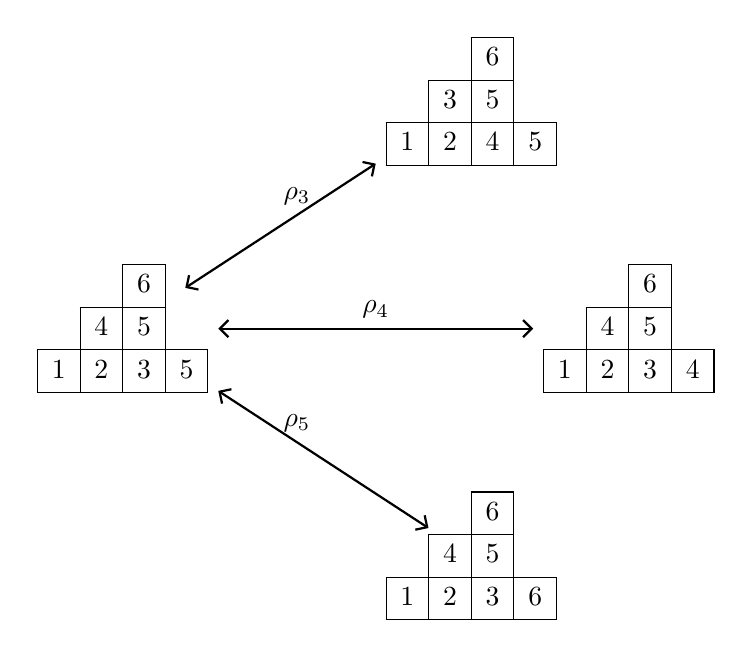
\begin{tikzpicture}
\node (A) {\ytableaushort{\none \none 6,\none 45,1235 } };
\node[above right = 1 and 2 of A] (B) {\ytableaushort{\none \none 6, \none 35, 1245}};
\node[ right = 4 of A] (C) {\ytableaushort{\none \none 6, \none 45,1234}};
\node[below right = 1 and 2 of A] (D) {\ytableaushort{\none \none 6, \none 45,1236}};
\path (A) edge[pilpil,shorten >=-0mm,shorten <=-5mm] node[above]{$\rho_3$} (B);
\path (A) edge[pilpil] node[above]{$\rho_4$} (C);
\path (A) edge[pilpil,shorten >=-8mm] node[above]{$\rho_5$} (D);
\end{tikzpicture}
\caption{The three increasing tableaux on the right are obtained from the increasing tableau at left by applying the indicated $K$-Bender-Knuth operators. The arrows point in both directions since each $K$-Bender-Knuth operator is involutive.}\label{fig:kbk}
\end{figure}

\begin{figure}[h]
\begin{center}
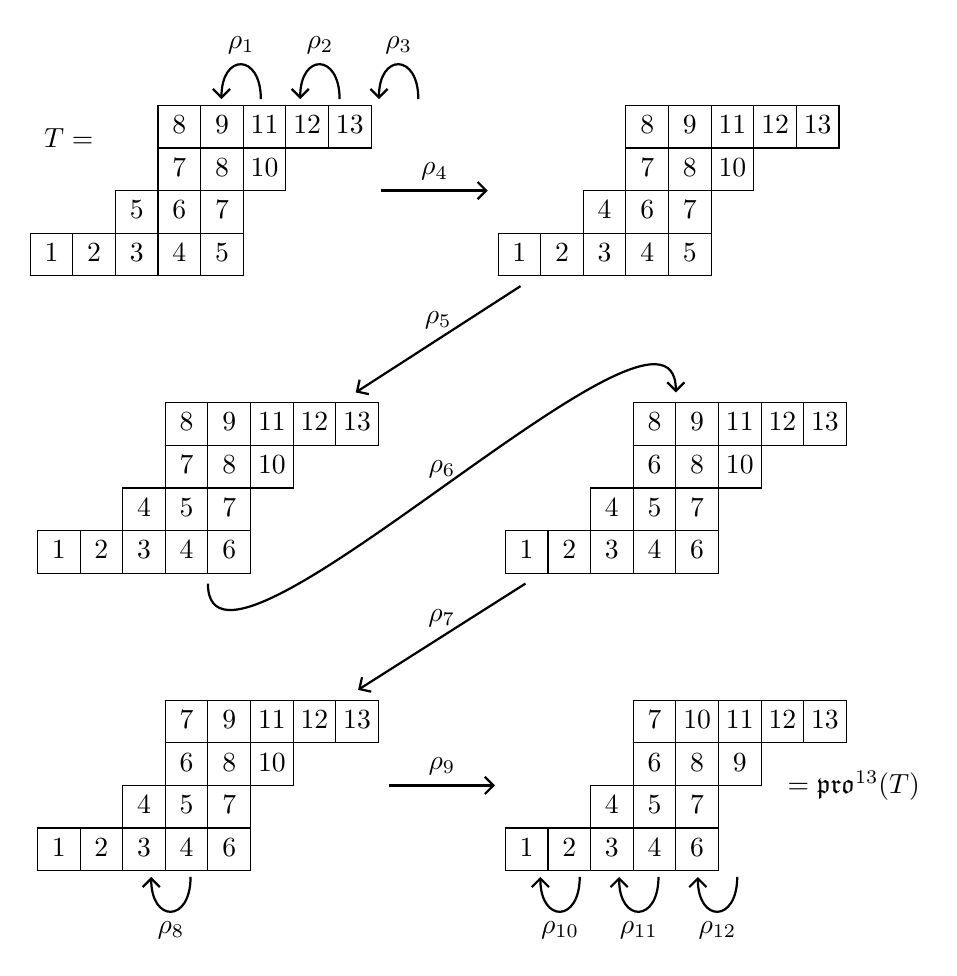
\begin{tikzpicture}
\node (T) {$T= \!\!\!\!\!\!\!$\hspace{-4mm}\ytableaushort{ \none \none \none 89{11}{12}{13},\none \none \none 78{10},\none \none 567, 12345}};
\node[right  = 1.35 of T] (T4) {\ytableaushort{ \none \none \none 89{11}{12}{13}, \none \none \none 78{10}, \none \none 467, 12345}};
\node[below  = 1.35 of T] (T5) {\ytableaushort{   \none \none \none 89{11}{12}{13}, \none \none \none 78{10},\none \none 457,12346}};
\node[right  = 1.35 of T5] (T6) {\ytableaushort{   \none \none \none 89{11}{12}{13}, \none \none \none 68{10},\none \none 457, 12346 }};
\node[below  = 1.35 of T5] (T7) {\ytableaushort{   \none \none \none 79{11}{12}{13},\none \none \none 68{10},\none \none 457, 12346 }};
\node[right  = 1.35 of T7] (T9) {\ytableaushort{  \none \none \none 7{10}{11}{12}{13},\none \none \none 689, \none \none 457, 12346 }};
\node[right = -1 of T9] (finishlabel) {$=\pro^{13}(T)$};
\node[below left = -.3 and -0.7 of T9] (fake1) {};
\node[below left = -.3 and -1.2 of T9] (fake2) {};
\node[below left = -.3 and -1.7 of T9] (fake3) {};
\node[below left = -.3 and -2.2 of T9] (fake4) {};
\node[below left = -.3 and -2.7 of T9] (fake5) {};
\node[below left = -.3 and -3.2 of T9] (fake6) {};
\node[above left = -.3 and -2.5 of T] (fake7) {};
\node[above left = -.3 and -3.0 of T] (fake8) {};
\node[above left = -.3 and -3.5 of T] (fake9) {};
\node[above left = -.3 and -4.0 of T] (fake10) {};
\node[above left = -.3 and -4.5 of T] (fake11) {};
\node[above left = -.3 and -5.0 of T] (fake12) {};
\node[below left = -.3 and -1.7 of T7] (fake13) {};
\node[below left = -.3 and -2.2 of T7] (fake14) {};
\path (T) edge[pil]  node[above]{$\rho_4$} (T4);
\path (T4) edge[pil] node[above]{$\rho_5$} (T5);
\draw[->, thick] (T5.south) .. node[above]{$\rho_6$} controls ([yshift=-3cm] T5) and ([yshift=3cm] T6) .. (T6.north);
\path (T6) edge[pil] node[above]{$\rho_7$} (T7);
\path (fake14) edge[pil,out=270,in=270,looseness=3] node[below]{$\rho_8$} (fake13);
\path (T7) edge[pil] node[above]{$\rho_9$} (T9);
\path (fake2) edge[pil, out=270, in=270, looseness=3] node[below]{$\rho_{10}$} (fake1);
\path (fake4) edge[pil, out=270, in=270, looseness=3] node[below]{$\rho_{11}$} (fake3);
\path (fake6) edge[pil, out=270, in=270, looseness=3] node[below]{$\rho_{12}$} (fake5);
\path (fake8) edge[pil, out=90, in=90, looseness=3] node[above]{$\rho_1$} (fake7);
\path (fake10) edge[pil, out=90, in=90, looseness=3] node[above]{$\rho_2$} (fake9);
\path (fake12) edge[pil, out=90, in=90, looseness=3] node[above]{$\rho_3$} (fake11);
\end{tikzpicture}
\end{center}
\caption{The calculation of the $K$-promotion $\pro^{13}(T)$ of the increasing tableau $T$ (on the Cayley-Moufang poset) through the action of the sequence of $K$-Bender-Knuth operators $\rho_1, \dots, \rho_{12}$.}\label{fig:promotion}
\end{figure}

\subsection{The equivariant bijection}\label{sec:equivariant}

Here, we observe that results of \cite{DPS} and \cite{Dilks.Striker.Vorland} enable us to study the rowmotion action $\Psi$ via the action of $K$-promotion on increasing tableaux.

%\begin{proposition}[{\cite[Corollary~3.28]{Dilks.Striker.Vorland}}]
%Let $P$ be a poset where the maximum length of a chain containing an element is the same for every element of $P$. Then Γ1(P, q) is in bijection with P × [q − rk(P)].
%\end{proposition}
%
%
%It is not hard to see that the posets we care about have this property. I think that by "is in bijection with", they actually mean "is isomorphic to".
%
%Then they have:

\begin{proposition}
Let $P \in \{ P_{CM}, P_F, P_p \}$ and $k \in \mathbb{Z}_{\geq 0}$.
There is an equivariant bijection between $\inc^{k+\rank(P)}(P)$ under $K$-promotion and $J(P \times {\bf k})$ under $\Psi$.
\end{proposition}
\begin{proof}
By \cite[Corollary~5.2]{Dilks.Striker.Vorland}, there is an equivariant bijection between the sets $\inc^{k+\rank(P)}(P)$ under $K$-promotion and $J(\Gamma_1(P,k+\rank(P)))$  under $\Psi$, where $\Gamma_1(P,k+\rank(P))$ is a poset constructed from $P$ in \cite[\textsection 3.1]{Dilks.Striker.Vorland}.
For any $\x \in P$, note that the maximal length $M$ of a chain through $\x$ is independent of $\x$. (Specifically, $M = 11$ for $P = P_{CM}$, $M= 17$ for $P = P_F$, and $M = 2p-1$ for $P = P_p$.)
Hence \cite[Corollary~3.28]{Dilks.Striker.Vorland} applies, and in these cases we have the isomorphism of posets $\Gamma_1(P,k+\rank(P)) \cong P \times {\bf k}$.
\end{proof}

\begin{corollary}\label{cor:multisets}
Let $P \in \{ P_{CM}, P_F, P_p \}$ and $m \in \mathbb{Z}_{\geq 0}$.
Then the multiset of cardinalities of $\Psi$-orbits on $J(P \times \mathbf{k})$ and the multiset of cardinalities of $\pro^{\rank(P)+ k+1}$-orbits on $\inc^{\rank(P)+ k+1}(\lambda)$ are equal. \qed
\end{corollary}
%\begin{proof}
%By Proposition~\ref{prop:bijection}, $\Omega$ is a bijection between $J(\lambda \times \mathbf{m})$ and $\inc^{\rank(\lambda)+ m+1}(\lambda^\star)$. By Proposition~\ref{prop:equivariant}, the orbit structure of $\pro^{\rank(\lambda)+ m+1}$ on $\inc^{\rank(\lambda)+ m+1}(\lambda^\star)$ is the same as the orbit structure of $\mot_{\mathrm{id},(1,1,-1)}$ on $J(\lambda \times \mathbf{m})$. By Proposition~\ref{prop:psi_is_toggle}, the action of $\Psi$ on $J(\lambda \times \mathbf{m})$ is the same as the action of $\mot_{\mathrm{id},(1,1,1)}$. By Proposition~\ref{prop:conjugate_actions}, $\mot_{\mathrm{id},(1,1,1)}$ and $\mot_{\mathrm{id},(1,1,-1)}$ induce the same multiset of orbit cardinalities on $J(\lambda \times \mathbf{m})$.
%\end{proof}

\subsection{Inflation and deflation}
Suppose $T \in \inc^m(\lambda)$ and consider $T$ as a strictly order-preserving map from $\lambda$ to the chain poset ${\bf m}$. We say that $T$ is {\bf gapless} if this map is surjective and {\bf gappy} otherwise. We write $\incgl^m(\lambda)$ for the subset of all gapless tableaux in $\inc^m(\lambda)$. Notice that the set 
\[
\incgl(\lambda) \coloneqq \coprod_{m} \incgl^m(\lambda)
\]
is finite. This fact will be critical to our proofs of Theorems~\ref{thm:exceptionals} and~\ref{thm:propeller}.

For $T \in \inc^m(\lambda)$, let $m_T \coloneqq |\mathrm{range}(T)|$ be the number of distinct labels in $T$. For each $m$, we define the {\bf deflation} map \[\deflate^m : \inc^m(\lambda) \to \coprod_{0 \leq n \leq m} \incgl^n(\lambda)\] by
\[
[\deflate^m(T)](\x) =
\# \{ h \in \mathrm{range}(T): h \leq T(\x) \} ,
\]
for $T \in \inc^m(\lambda)$ and $\x \in \lambda$. Note that $\deflate^m(T) \in \incgl^{m_T}(\lambda)$ and that $m_T \leq m$.

For positive integers $j$ and $k$, let $\binom{[j]}{k}$ denote the collection of binary vectors of length $j$ with $k$ $1$'s. We now define the {\bf content vector} function 
\[
 \content^m : \inc^m(\lambda) \to \{ 0, 1\}^m = \coprod_{0 \leq  n \leq m} \binom{[m]}{n}
 \] 
 by 
\[
\content^m(T) = (c_1, \dots, c_m),
\] 
where $c_i = 1$ if $i \in \mathrm{range}(T)$ and $c_i = 0$ if $i \notin \mathrm{range}(T)$. Note that this definition of content differs from the usual notion of content for semistandard tableaux in that here we do not care about the multiplicity of a label, but only its presence or absence.

\begin{example}\label{ex:deflate}
If $T = \ytableaushort{456,125} \in \inc^7(2 \times 3)$, then the deflation of $T$ is \[\deflate^7(T) = \ytableaushort{345,124} \in \incgl^5(2 \times 3).\] The content vector of $T$ is $\content^7(T) = (1,1,0,1,1,1,0) \in \binom{[7]}{5} \subset \{0,1\}^7$.
\end{example}
Now if $\deflate^m(T) \in \incgl^n(\lambda)$, then $\content^m(T) \in \binom{[m]}{n}$. We denote by $\compress^m$ the product map
\[
\compress^m \coloneqq (\deflate^m,\content^m).
%: \inc^m(\lambda) \to \coprod_{0 \leq n \leq m} \left( \incgl^n(\lambda) \times \binom{[m]}{n} \right).
\] 
\begin{theorem}\label{thm:compressbijective} The map 
\[
\compress^m : \inc^m(\lambda) \to \coprod_{0 \leq n \leq m} \left( \incgl^n(\lambda) \times \binom{[m]}{n} \right)
\]
 is bijective.
\end{theorem}
\begin{proof}
%We claim that $W = (W_1,W_2)$ is an injection $\text{Inc}^q(\lambda) \rightarrow \coprod_{M \leq N+1} \text{Inc}^{M}(\lambda)\times  (\mathbb{Z}/2\mathbb{Z})^{q}$. 
A two-sided inverse for $\compress^m$ is given as follows. For any nonnegative integer $j$, let $[j]$ denote the set $\{1, 2, \dots, j\}$.
For a binary vector $v \in \{0,1\}^m$, let $N_v$ be the number of $1$'s in $v$, and define a {\bf vector inflation} map \[\inflate^m_v : [N_v] \to [m]\] by
\[ \inflate^m_v(k) = \min \bigg\lbrace n \in [m]:   \sum_{\ell = 1}^n v\lbrace \ell \rbrace = k \bigg\rbrace.\] (We use curly braces $``\{\}"$ throughout the paper to denote vector components.) An integer $j \in [m]$ is in the range of $\inflate^m_v$ if and only if $v\lbrace j \rbrace = 1$. Therefore
\begin{align*}
[\inflate^m_{\content^m(T)} \circ \deflate^m(T)](\x) &= \min \bigg\lbrace n \in [m]:    \# \{ h \in \mathrm{range}(T): h \leq n \} = [\deflate^m(T)](\x) \bigg\rbrace \\ &= T(\x). 
\end{align*} Now define the {\bf tableau inflation} map 
\[
\tinflate^m : \coprod_{0 \leq n \leq m} \left( \incgl^n(\lambda) \times \binom{[m]}{n} \right) \to \inc^m(\lambda)
\] 
by 
\[
\tinflate^m(S,v) = \inflate^m_v \circ S.
\]
Say $(S,v) \in \incgl^n(\lambda) \times \binom{[m]}{n}$. Since $S$ is surjective onto $[n]$ and $\inflate^m_v$ maps $[n]$ onto the indices of nonzero components in $v$, $\content^m \circ \tinflate^m(S,v) = v$.  Also,
\begin{align*}
 [\deflate^m(\inflate^m_v  \circ S)](\x) &= \# \{ h \in \mathrm{range}(\inflate^m_v \circ S): h \leq \inflate^m_v \circ S(\x) \} \\  
 &= \# \{ h: v\{h\} \neq 0 \text{ and } \sum_{\ell = 1}^h v\{\ell\} \leq S(\x)  \} \\
 &= S(\x).
\end{align*}
Therefore, $\tinflate^m$ is a two-sided inverse for $\compress^m$.
\end{proof} 
\begin{example}\label{ex:reinflate}
Let $v = (1,1,0,1,1,1,0) \in \{0,1\}^7$. Then, $N_v = 5$ and the map $\inflate^7_v : [5] \to [7]$ is given by 
\begin{align*}
\inflate^7_v(1) &= 1, \\
\inflate^7_v(2) &= 2, \\
\inflate_v^7(3) &= 4, \\
\inflate_v^7(4) &= 5, \\
\inflate_v^7(5) &= 6. 
\end{align*}
Now, for $S = \ytableaushort{345,124}$, we have $\tinflate^7(S,v) = \inflate^7_v \circ S = \ytableaushort{456,125}$. Note that this process has recovered the tableau $T$ of Example~\ref{ex:deflate} from $S=\deflate^7(T)$ and $v=\content^7(T)$.
\end{example}

\subsection{Interaction between $K$-promotion and deflation}
By determining the relation between the maps $\compress^m$ and $\pro^m$, we will show that $\pro^m$ is controlled by its action on gapless increasing tableaux. The power of this observation is that there are only finitely-many gapless increasing tableaux of any fixed shape $\lambda$. Thus a finite amount of data governs the action of $\pro^m$ on $\inc^m(\lambda)$ for all $m$.


To establish this relation, we first need to introduce a different characterization of $\pro^m$. Let $\rep_{1 \rightarrow \bullet}$ be the operator on $\inc^m(\lambda)$ that replaces each instance of $1$ by $\bullet$. Let $\swap_n$ be the operator that finds all edge-connected components containing $\bullet$ and $n$, leaves trivial components unchanged, and switches $n$ and $\bullet$ in nontrivial connected components. Let $\rep_{\bullet \rightarrow m+1}$ replace each instance of $\bullet$ with $m+1$. Finally, let $\decr$ be the operator that decrements each label by $1$. Then \cite[Proposition~2.4]{DPS} gives the following equivalent characterization of the operation of $K$-promotion on $\inc^m(\lambda)$: 
\begin{equation}\label{eq:kprodef2}
\pro^m = \decr \circ \rep_{\bullet \rightarrow m+1} \circ \swap_m \circ \cdots \circ \swap_2 \circ \rep_{1 \rightarrow \bullet}.
\end{equation}
 This was, in fact, the original definition of $K$-promotion introduced in \cite{Pechenik}. An example of computing $K$-promotion via this process is shown in Figure~\ref{fig:promotion_via_swaps}.
 
 \begin{figure}[h]
 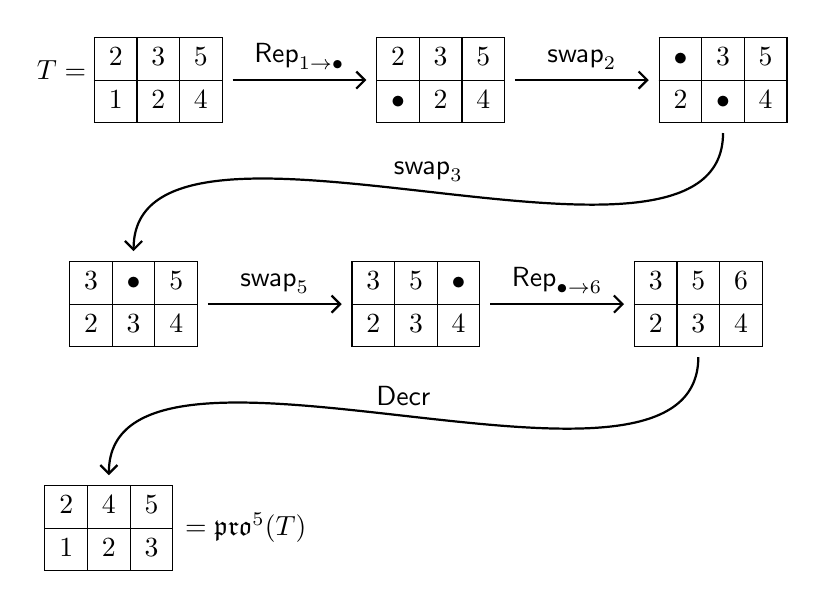
\begin{tikzpicture}
\node (T) {$T= \;$\ytableaushort{ 235,124}};
\node[right  = 1.7 of T] (T4) {\ytableaushort{ 235, \bullet 24}};
\node[right  = 1.7 of T4] (T5) {\ytableaushort{   \bullet 35, 2 \bullet 4}};
\node[below right  = 1.5 and -2.2 of T] (T6) {\ytableaushort{   3 \bullet 5, 234 }};
\node[right  = 1.7 of T6] (T7) {\ytableaushort{   35 \bullet, 234 }};
\node[right  = 1.7 of T7] (T9) {\ytableaushort{  356,234 }};
\node[below right = 1.5 and -2.2 of T6] (T10) {\ytableaushort{245,123}};
\node[right = -0.1 of T10] (pro) {$=\pro^5(T)$};
\path (T) edge[pil]  node[above]{$\rep_{1 \rightarrow \bullet}$} (T4);
\path (T4) edge[pil] node[above]{$\swap_2$} (T5);
\draw[->, thick] (T5.south) .. node[above]{$\swap_3$} controls ([yshift=-3cm] T5) and ([yshift=3cm] T6) .. (T6.north);
\draw[->, thick] (T9.south) .. node[above]{$\decr$} controls ([yshift=-3cm] T9) and ([yshift=3cm] T10) .. (T10.north);
\path (T6) edge[pil] node[above]{$\swap_5$} (T7);
\path (T7) edge[pil] node[above]{$\rep_{\bullet \rightarrow 6}$} (T9);
\end{tikzpicture}
\caption{The calculation of the $K$-promotion $\pro^5(T)$ of the increasing tableau $T$ through the action of a sequence of swaps.}\label{fig:promotion_via_swaps}
 \end{figure}

Using this characterization, we give names to the intermediate products of $\pro^m$.
For $T \in \inc^m(\lambda)$ and $n \leq m$, we define the tableau $T^{(n)}: \lambda \rightarrow \lbrace 2, \dots, m, \bullet \rbrace$ by 
\[T^{(n)} \coloneqq \swap_n \circ \cdots \circ \swap_2 \circ \rep_{1 \rightarrow \bullet}(T)\] for $n > 1$ and $T^{(1)} \coloneqq \rep_{1 \rightarrow \bullet}(T)$. We define the associated order ideal 
\[
\lambda \left( T^{(n)} \right) \coloneqq \left( T^{(n)} \right)^{-1}(\{2,\dots,n\})
\]
 to be the set of boxes of $T^{(n)}$ containing entries from $\{2,\dots,n\}$. Finally, define 
 \[
 T_n \coloneqq T^{(n)} \vert_{\lambda \left( T^{(n)} \right) }.
 \]
  Intuitively, $T^{(n)}$ shows $T$ at the point in $K$-promotion at which the boxes labeled $2$ through $n$ have been acted upon by $\swap$ operators, while $T_n$ is the restriction of $T^{(n)}$ to this subset of boxes. Examples of these intermediate tableaux appear in Figure~\ref{fig:restricted_promotions}. 
  
  
\begin{figure}[h]
%\includegraphics[scale=.35]{lemma_4p2.jpg}
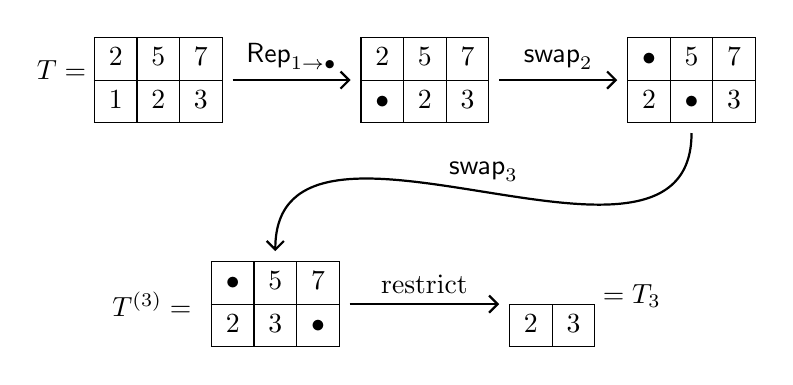
\begin{tikzpicture}
\node (T) {$T = \ytableaushort{257,123}$};
\node[right=1.5 of T] (D) {\ytableaushort{257,\bullet 23}};
\node[right = 1.5 of D] (T2) {\ytableaushort{\bullet 57,2 \bullet 3}};
\node[below right = 1.5 and -0.4 of T] (T3) {\ytableaushort{\bullet 5 7,23 \bullet}};
\node[left = 0 of T3] (mytag) {$T^{(3)}=$};
\node[right = 1.9 of T3] (Tres3) {\ytableaushort{\none,23} $\; = T_3$};
%\node[above left = -.2 and -0.7 of D] (fake1) {};
%\node[above left = -.2 and -2.0 of D] (fake2) {};
\path (T) edge[pil] node[above]{$\rep_{1 \rightarrow \bullet}$} (D);
\path (D) edge[pil] node[above]{$\swap_2$} (T2); 
\path (T3) edge[pil] node[above]{restrict} (Tres3);
\draw[->, thick] (T2.south) .. node[above]{$\swap_3$} controls ([yshift=-3cm] T2) and ([yshift=3cm] T3) .. (T3.north);
%\path (fake2) edge[pil, out=90, in=90, looseness=1.5] node[above]{$\swap_1$} (fake1);
\end{tikzpicture}
\caption{The tableau $T^{(3)}$ is obtained from $T$ by applying in sequence the operations 
$\rep_{1 \rightarrow \bullet}$, $\swap_2$, and $\swap_3$. 
We then obtain $T_3$ from $T^{(3)}$ by restricting to 
those boxes with labels less than or equal to $3$. The order ideal
 $\lambda \left( T^{(3)} \right)$ is the 
shape of the tableau $T_3$. }\label{fig:restricted_promotions}
\end{figure}

%-- not obvious that $\lambda$  is a shape but don't think need this here -- 
We use these intermediate products to characterize the action of $K$-promotion on gappy tableaux. 

\begin{lemma}\label{lem:deflation_commutation}
For $T \in \inc^m(\lambda)$, if $\content^m(T) \lbrace 1 \rbrace = 1$, then
\begin{equation}\label{eq:deflation_commutation}
\deflate^m \circ \pro^m(T) = \pro^{m_T} \circ \deflate^m(T).
\end{equation}
If $\content^m(T) \lbrace 1 \rbrace = 0$, then $\pro^m(T) = \decr(T)$. 
\end{lemma} 
This result is intuitive, since after the ``initialization'' that replaces $1$s with $\bullet$s, the steps of $K$-promotion depend essentially on the relative magnitude of the labels. A careful proof requires the following technical lemmas (Lemmas~\ref{lem:bullet_placement} and ~\ref{lem:gappy_promotion}). 
\begin{lemma} \label{lem:bullet_placement}
Let $T \in \inc^m(\lambda)$ with $\content^m(T) \lbrace 1 \rbrace = 1$. Let $i_j = \inflate^m_{\content^m(T)}(j)$ for $1 \leq j \leq m_T$. Then, for all $\x \in \lambda$ and $1 \leq j \leq m_T$, we have
 \begin{equation}\label{eq:gappy_promotion2}
\deflate^m(T)^{(j)}(\x) = \bullet \text{ if and only if } T^{(i_j)}(\x) = \bullet.
\end{equation}
\end{lemma}
\begin{proof} We proceed by induction on $j$. Fix $T \in \inc^m(\lambda)$  with $\content^m(T) \lbrace 1 \rbrace = 1$. In the base case $j = 1$,  $T^{(i_1)} = T^{(1)} = \rep_{1 \rightarrow \bullet}(T)$ has $\bullet$ in exactly those boxes $\x \in \lambda$ such that $T(\x) = 1$. On the other hand, $\deflate^m(T)^{(1)} =  \rep_{1 \rightarrow \bullet}(\deflate^m(T))$ has $\bullet$ in exactly those boxes $\x \in \lambda$ such that $\deflate^m(T)(\x) = 1$. But since $\content^m(T) \lbrace 1 \rbrace = 1$, $\deflate^m(T)(\x) = 1$ if and only if $T(\x) = 1$. 


Now, say the lemma holds for all such $T$ in the case $j < t$. First consider the case where $T^{(i_t)}(\x) = \bullet$ and $T^{(i_{t-1})}(\x) \neq \bullet$. This is equivalent to the statement that $T^{(i_{t-1})}(\x) = i_t$ and $T^{(i_{t-1})}(\x') = \bullet$ for some $\x'$ adjacent to $\x$. But since $\rep_{1 \rightarrow \bullet}$ and $\swap_j$ for  $j \leq i_{t-1}$ only act on elements of $T$ labeled with $\bullet$'s or values less than or equal to $i_{t-1}$, $T^{(i_{t-1})}(\x) = i_t$ implies that $T(\x) = i_t$. This is, in turn, equivalent by Theorem~\ref{thm:compressbijective} to the statement $\deflate^m(T)(\x) = t$, implying that $\deflate^m(T)^{(t-1)}(\x) = t$. Additionally, by the inductive hypothesis, $T^{(i_{t-1})}(\x') = \bullet$ if and only if $\deflate^m(T)^{(t-1)}(\x') = \bullet$. Therefore, the conditions of this case are equivalent to the conditions $\deflate^m(T)^{(t)}(\x) = \bullet$ and $\deflate^m(T)^{(t-1)}(\x) \neq \bullet$, as desired. 

Consider the other possible case, where $T^{(i_t)}(\x) = \bullet$ and $T^{(i_{t-1})}(\x) = \bullet$. This scenario is equivalent to the statement that $T^{(i_{t-1})}(\x) = \bullet$ and there is no $\x'$ adjacent to $\x$ such that $T^{(i_{t-1})}(\x') = i_t$. By similar reasoning as in the previous case, the second condition is equivalent to the statement that there is no $\x'$ adjacent to $\x$ with $T(\x') = i_t$. This statement is, in turn, equivalent to saying that there is no $\x'$ adjacent to $\x$ with $\deflate^m(T)(\x') = \deflate^m(T)^{(t-1)}(\x') = t$. Since $\deflate^m(T)^{(t-1)}(\x) = \bullet$ by the inductive hypothesis, the conditions of this case are finally equivalent to the conditions that $\deflate^m(T)^{(t)}(\x) = \bullet$ and $\deflate^m(T)^{(t-1)}(\x) = \bullet$, and we are done.
\end{proof}
\begin{lemma} \label{lem:gappy_promotion}
Take $T$ and $i_1, \ldots, i_{m_T}$ as in Lemma~\ref{lem:bullet_placement}. Then for $1 \leq j \leq m_T$, 
\begin{equation}\label{eq:gappy_promotion}
 \tinflate^m \Big( \deflate^m(T)_j, \content^m(T) \Big) = T_{i_j}.
\end{equation}
That is, the two sides are identical functions on the same domain. 
\end{lemma}
\begin{remark}The statement of the lemma involves a slight abuse of notation, since in general $\content^m(T)$ has more nonzero entries than $\lambda(\deflate^m(T)^{(j)})$ has boxes. This does not present an issue, since $\tinflate^m$ extends to a well-defined operator on vectors with excess $1$s.
\end{remark}
\begin{proof}  We proceed again by induction on $j$. The base case $j=1$ is trivial, since for any $T \in \inc^m(\lambda)$, $\lambda \left( \deflate^m(T)^{(1)} \right)$ and $\lambda \left( T^{(1)} \right)$ are both the empty order ideal.
%To establish the base case for this $T$, note that all numerical entries of $\rep_{1 \rightarrow \bullet}(T)_{1}$ are at least $2$. Therefore, $\swap_1$ acts trivially, $\lambda(T^{(1)}) = \emptyset$, and $T_1 = T_{i_1}$ is the empty tableau. The same reasoning shows that $\lambda(\deflate^q(T)^{(1)})$ is the empty tableau. %

Now, assume that the lemma holds for all increasing tableaux $T$ in the case $j < t$. We first analyze the left side of Equation~(\ref{eq:gappy_promotion}). Take $\x \in \lambda\left( \deflate^m(T)^{(t)} \right)$. If $\x \in \lambda\left( \deflate^m(T)^{(t-1)} \right)$, then 
$[\deflate^m(T)^{(t-1)}](\x) \leq t-1$ and hence
\[
\left[ \swap_{t}(\deflate^m(T)^{(t-1)})\right](\x) = \deflate^m(T)^{(t-1)}(\x).
\]
 If instead
 \[\x \in \lambda\left(\deflate^m(T)^{(t)}\right) \setminus \lambda\left(\deflate^m(T)^{(t-1)}\right),\]
  then either $[\deflate^m(T)^{(t-1)}](\x) = \bullet$ or $[\deflate^m(T)^{(t-1)}](\x) = t$. In the former case, there must be a box $\x'$ adjacent to $\x$ such that $[\deflate^m(T)^{(t-1)}](\x') = t$. In the latter case, we must have that for all boxes $\x'$ adjacent to $\x$, $[\deflate^m(T)^{(t-1)}](\x') \neq \bullet$. 

Now, we analyze the right side of Equation~(\ref{eq:gappy_promotion}). Take $\x \in \lambda\left( T^{(i_t)} \right)$.   If $\x \in \lambda \left(T^{(i_{t-1})} \right)$, then $\x \in \lambda(\deflate^m(T)^{(t-1)}) \subseteq \lambda(\deflate^m(T)^{(t)})$ by the inductive hypothesis. Further, this implies that $T^{(i_{t-1})}(\x) \leq i_{t-1}$,  and so we have
\[
\left[ \swap_{\ell+1} \left(T^{(\ell)} \right) \right](\x) = T^{(\ell)}(\x)
\]
 for all $i_{t-1} \leq \ell$. Therefore by the previous paragraph and the inductive hypothesis,
 \[ T^{(i_t)}(\x) = T^{(i_{t-1})}(\x) = \inflate^m_{\content^m(T)} \circ \deflate^m(T)^{(t-1)}(\x) =  \inflate^m_{\content^m(T)} \circ \deflate^m(T)^{(t)}(\x). \] This shows that Equation~(\ref{eq:gappy_promotion}) holds at $\x$. If $\x \in \lambda \left(T^{(i_{t})} \right) \setminus \lambda \left(T^{(i_{t-1})} \right)$, then $i_{t-1} < T^{(i_{t})}(\x) \leq i_t$. Thus, we must have that $T^{(i_{t})}(\x) = i_{t}$, since the $\swap$ operators do not change the content of a tableau. Therefore, either $T^{(i_{t-1})}(\x) = \bullet$ or $T^{(i_{t-1})}(\x) =  T(\x) = i_{t}$. In the former case, there must be a box $\x'$ adjacent to $\x$ such that $T^{(i_{t-1})}(\x') = T(\x') = i_{t}$. This occurs exactly when $\deflate^m(T)^{(t-1)}(\x') = \deflate^m(T)(\x') = t$. In the latter case, there is no $\x'$ adjacent to $\x$ such that $T^{(i_{t-1})}(\x') = \bullet$. Since we have assumed that  $\content^m(T) \lbrace 1 \rbrace = 1$, Lemma~\ref{lem:bullet_placement} implies that this occurs exactly when  $\deflate^m(T)^{(t-1)}(\x') \neq \bullet$ for every box $\x'$ adjacent to $\x$. Therefore each of these conditions is equivalent to the corresponding condition from the previous paragraph. 
 
Putting these facts together, we have shown that $\lambda \left(T^{(i_j)} \right) = \lambda \left(\deflate^m(T)^{(j)} \right)$ for all $j$, and that $\deflate^m(T)_j(\x) = h$ if and only if $T_j(\x) = \inflate^m_{\content^m(T)}(h)$. 
\end{proof}

%\begin{remark}
%As a corollary to Lemma~\ref{lem:gappy_promotion}, one can show that each $T_j$ is, in fact, in $\inc^m \left(\lambda \left( T^{(j)} \right) \right)$. However, we do not need this observation here.
%\end{remark}
%

%\begin{proof} Since $\content^m(T) \lbrace 1 \rbrace = 1$, $\deflate^m(T)$ and $T$ are labelled by $1$ in the same boxes, and therefore $\rep_{1 \rightarrow \bullet}(\deflate^m(T))$ and $\rep_{1 \rightarrow \bullet}(T)$ have $\bullet$s in the same boxes. 
%
%Now each operation $\swap_j$ either leaves the tableau unchanged or exchanges $\bullet$s and numerical values in a way that depends only on the relative magnitude of the labels of the tableau. Since $\deflate^m$ preserves the relative magnitude of labels, it therefore clear that the relative magnitudes of the labels of $\rep_{\bullet \rightarrow m+1} \circ \swap_m \circ ... \circ \swap_2 \circ \rep_{1 \rightarrow \bullet} (T)$ are the same as the relative magnitudes of the labels of  $\rep_{\bullet \rightarrow {m_T}+1} \circ \swap_{m_T} \circ ... \circ \swap_2 \circ \rep_{1 \rightarrow \bullet} (\deflate^m(T))$.  
%
%Since $\decr$ does not change the relative order of labels, it follows that $\pro^m(T)$ and $\pro^{m_T} \circ \deflate^m(T)$ have the same relative magnitudes of labels. But $\pro^m$ does not change the content vector of $T$, so $\inflate^m_{\content^m(T)} \circ \pro^{m_T} \circ \deflate^m(T) = \pro^m(T)$. 
%\end{proof}
\begin{proof}[Proof of Lemma~\ref{lem:deflation_commutation}]
If $\compress^m(T)\lbrace 1 \rbrace = 0$, then $\rep_{1 \rightarrow \bullet}(T) = T$. But then $\swap_\ell(T) = T$ for all $\ell$, since there are no nontrivial short ribbons containing the labels $\bullet$ and $\ell$. Also, $\rep_{\bullet \rightarrow 1}(T) = T$, since there is no $\bullet$ label in $T$. Therefore, $\decr$ is the only operator in Equation~(\ref{eq:kprodef2}) that acts nontrivially on $T$. 


Say otherwise that $\compress^m(T)\lbrace 1 \rbrace = 1$. By Equation~(\ref{eq:kprodef2}), we must show that
\begin{align*}
\deflate^m \circ &\decr \circ \rep_{\bullet \rightarrow m+1} \circ \swap_m \circ \cdots \circ \swap_2\circ \rep_{1 \rightarrow \bullet} (T) = \\
 & \decr \circ \rep_{\bullet \rightarrow m_T+1} \circ \swap_{m_T} \circ \cdots \circ \swap_2 \circ \rep_{1 \rightarrow \bullet} \circ \deflate^m (T). 
\end{align*}
Say $\x \not \in \lambda(T^{(m)})$; that is,  $T^{(m)}(\x) = \bullet$.  Then,
\[
[\decr \circ \rep_{\bullet \rightarrow m+1} \circ \swap_m \circ \cdots \circ \swap_2 \circ \rep_{1 \rightarrow \bullet} (T)](\x) = m.
\]
Now by \cite[Lemma~2.1]{DPS}, the content vector of  
\[
\decr \circ \rep_{\bullet \rightarrow m+1} \circ \swap_m \circ \cdots \circ \swap_2 \circ \rep_{1 \rightarrow \bullet} (T) = \pro^m(T)
\]
 is a cyclic rotation by one of the content vector of $T$. This implies that there are the same number of distinct labels in the content vector of $\pro^m(T)$, namely $m_T$, and, since $m$ is included, it must be the greatest such label, so 
 \[
 [\deflate^m \circ \decr \circ \rep_{\bullet \rightarrow m+1} \circ \swap_m \circ \cdots \circ \swap_2 \circ \rep_{1 \rightarrow \bullet} (T)](\x) = m_T.
 \]
  On the other hand, since Lemma~\ref{lem:bullet_placement} implies that $\x \not \in \lambda(\deflate^m(T)^{(m_T)})$, we have
  \[
  [\decr \circ \rep_{\bullet \rightarrow m_T + 1} \circ \swap_{m_T} \circ \cdots \circ \swap_2 \circ \rep_{1 \rightarrow \bullet} \circ \deflate(T)](\x) = m_T.
  \] 

Now say $\x \in \lambda(T^{(m)})$ and let $i_1, \ldots, i_{m_T}$ be as in Lemma~\ref{lem:bullet_placement}. We observe that since $\swap_\ell$ does not affect the tableau $\swap_{m_T} \circ \cdots \circ \swap_2 \circ \rep_{1 \rightarrow \bullet} (T)$ for $\ell > i_{m_T}$, we have that
\[ (\swap_m \circ \cdots \circ \swap_2 \circ \rep_{1 \rightarrow \bullet}( T ))_m = (\swap_{i_{m_T}} \circ \cdots \circ \swap_2 \circ \rep_{1 \rightarrow \bullet}( T ))_{i_{m_T}}.  \]
Therefore, it follows from Lemma~\ref{lem:gappy_promotion}, taking $j = m_T$, that 
\[ (\swap_m \circ \cdots \circ \swap_2 \circ \rep_{1 \rightarrow \bullet}( T ))_m = \inflate^m_{\content^m(T)} \circ (\swap_{m_T} \circ \cdots \circ   \swap_2  \circ \rep_{1 \rightarrow \bullet} \circ \deflate^m(T)_{m_T}). \]

Now, since $\x \in \lambda(T^{(m)})$, we have that $T^{(m)}(\x) = \ell$ for $\ell \in \{2,3,\dots,m\}$. This implies that $\ell = i_j$ for some $2 \leq j \leq m_T$. Then, 
\[
\decr \circ \rep_{\bullet \to m+1} \circ \swap_m \circ \cdots \circ \swap_2 \circ \rep_{1 \rightarrow \bullet} (T)(\x) = i_j-1.
\]
Because $\content^m(T) \lbrace 1 \rbrace = 1$ and the content vector shifts cyclically, this implies that 
 \[
 [\deflate^m \circ \decr \circ \rep_{\bullet \rightarrow m+1} \circ \swap_m \circ \cdots \circ \swap_2 \circ \rep_{1 \rightarrow \bullet} (T)](\x) = j-1.
 \]
  On the other hand, 
  \[
  [\swap_{m_T} \circ \cdots \circ \swap_2 \circ \rep_{1 \rightarrow \bullet} \circ \deflate^m(T)](\x) = j,
  \]
   so 
   \[
   [ \pushQED{\qed} \decr \circ \rep_{\bullet \rightarrow m_T + 1} \circ \swap_{m_T} \circ \cdots \circ \swap_2 \circ \rep_{1 \rightarrow \bullet} \circ  \deflate^m(T)](\x) = j-1. \qedhere \popQED \] \let\qed\relax
\end{proof}

\subsection{Computation of period}\label{sec:period} We use Lemma~\ref{lem:deflation_commutation} to relate the period of $T \in \inc^m(\lambda)$ under $\pro^m$ to data concerning $\deflate^m(T)$. Let 
\[\Sigma^m : \lbrace 0,1\rbrace^m \rightarrow \lbrace 0,1\rbrace^m\]
 be the cyclic rotation defined by 
 \[
 \Sigma^m(v_1, \dots, v_m) = (v_2, \dots, v_m, v_1)
 \]
  for $(v_1, \dots, v_m) \in \lbrace 0,1 \rbrace^m$. 
  
\begin{theorem}\label{thm:periodthm}
Fix $T \in \inc^m(\lambda)$. Let $\tau$ be the the period of $\pro^{m_T}$ on $\deflate^m(T)$ and $\ell$ be the period of $\Sigma^m$ on $\content^m(T)$. Then, the period of $\pro^m$ on $T$ is \[\frac{\ell  \tau}{\mathrm{gcd}(\ell m_T / m,\tau)}. \]
\end{theorem} 
    
  \begin{proof}
Define
  \[
  K^m: \coprod_{n \leq m}\incgl^n(\lambda) \times \binom{[m]}{n} \rightarrow \coprod_{n \leq m}\incgl^n(\lambda) \times \binom{[m]}{n}
  \] by
\[
K^m(S,v) =
\begin{cases}
    \big( \pro^{N_S}(S),\Sigma^m(v) \big),  & \text{if } v\{1\} = 1; \\        
   \big( S,\Sigma^m(v) \big), & \text{otherwise.}
\end{cases}
\]
We first show that, for $T \in \inc^m(\lambda)$,
\begin{equation}\label{eq:k_commutes}
\compress^m \circ \pro^m(T) = K^m \circ \compress^m(T).
\end{equation}
Let $\pi_1$ be the projection onto the first factor of $\coprod_{n \leq m}\incgl^n(\lambda) \times \binom{[m]}{n}$ and $\pi_2$ the projection onto the second factor. It is immediate from the definitions that \[ \pi_2(K^m \circ \compress^m(T)) = \Sigma^m \circ \content^m(T).\] But by \cite[Lemma~2.1]{DPS},
\[  \Sigma^m \circ \content^m(T) = \content^m \circ \pro^m(T) = \pi_2(\compress^m \circ \pro^m(T)).\] Thus, the two sides of Equation~(\ref{eq:k_commutes}) are equal in the second factor.  

We now show that Equation~(\ref{eq:k_commutes}) holds in the first factor. Let \[ w \coloneqq \content^m(T) = \pi_2(\compress^m(T)). \]  By Theorem~\ref{thm:compressbijective}, we can write
\[ T = \tinflate^m(\deflate^m(T), w).\] 
If $w\lbrace 1 \rbrace = 1 $, then
\begin{align*}
\pi_1(\compress^m \circ \pro^m(T)) &= \deflate^m \circ \pro^m(T) \\
&= \pro^{m_T} \circ \deflate^m (T) &\text{Lemma~\ref{lem:deflation_commutation}, $w\lbrace 1 \rbrace = 1$} \\
&= \pro^{m_T} \circ \pi_1 \circ \compress^m(T) \\ 
&= \pi_1(K^m \circ \compress^m(T)) &\text{because $w\lbrace 1 \rbrace = 1$.}
\end{align*}
On the other hand, if $w \lbrace 1 \rbrace = 0$, then 
\begin{align*}
\pi_1(\compress^m \circ \pro^m(T)) &= \deflate^m \circ \pro^m(T) \\
&= \deflate^m(T) &\text{by Lemma~\ref{lem:deflation_commutation}, $w \lbrace 1 \rbrace = 0$} \\
&= \pi_1 ( \compress^m(T) ) \\
&= \pi_1 ( K^m \circ \compress^m(T)) &\text{because $w\lbrace 1 \rbrace = 0$.}
\end{align*}
This completes the proof of Equation~(\ref{eq:k_commutes}).

Now, since $\compress^m$ is a bijection by Theorem~\ref{thm:compressbijective}, $(\pro^m)^{\circ n}(T) = T$ exactly when $\compress^m \circ (\pro^m)^{\circ n}(T) = \compress^m \circ T$. So, by Equation~(\ref{eq:k_commutes}), we are reduced to determining which powers $n$ of $K^m$ stabilize $\compress^m(T)$.
 

 
Say $(K^m)^{\circ n}(\compress^m(T)) = \compress^m(T)$. Applying $\pi_2$ to both sides, we have \[ (\Sigma^m)^{\circ n}(\content^m(T)) = \content^m(T), \] so $n$ is a multiple of $\ell$. Hence, $n = t \ell$ for some integer $t \in \mathbb{Z}$.  Applying instead $\pi_1$ to both sides, we have \[ (\pro^m)^{\circ n'}(\deflate^m(T)) = \deflate^m(T), \] where 
\begin{align*}
n' &\coloneqq n - \# \{ 0 \leq j \leq n-1 : \pi_2 ((K^m)^{\circ j} \circ \compress^m(T)) \lbrace 1 \rbrace = 0\} \\
&= n - \#  \{ 1 \leq i \leq n : \content^m(T) \lbrace i \mod m \rbrace = 0\}.
\end{align*}
Let $r$ be the number of $0$s among the first $\ell$ entries of $\content^m(T)$. Then, $n' = t(\ell - r)$. Since $(\pro^m)^{\circ n'}$ fixes $\deflate^m(T)$, $n'$ is a multiple of $\tau$. Hence, $n' = s \tau$ for some integer $s$, and so $n = n' + tr = s\tau + tr$.

Thus, we have $(K^m)^{\circ n}  \circ \compress^m(T) = \compress^m(T)$ if and only if $n = t \ell = s \tau + t  r$ for some integers $s$ and $t$. Hence, the order of $\pro^m$ on $T$ is the least positive integer $h$ that can be simultaneously written in the forms $h = t \ell$ and $h=s \tau + t r$ for the same value of $t$. But $t \ell = s\tau + tr$ implies $t(\ell-r) = s\tau$. Since $0 \leq r < \ell$, the least such $h$ is clearly achieved when $t$ is minimal, i.e.\ when $t(\ell-r)$ is the least common multiple of $\ell-r$ and $\tau$. Thus, $h$ can be expressed as 
\begin{equation}\label{eq:period}
h = t \ell = \frac{\ell \, \text{lcm}(\ell-r,\tau)}{\ell-r} = \frac{\ell \tau}{\text{gcd}(\ell-r,\tau)}.
\end{equation}

Finally, observe that $r = \frac{\ell (m-m_T)}{m}$, so that \[ \ell - r = \frac{\ell m_T}{m}.\]
Therefore,
\[ h = \frac{\ell \tau}{\text{gcd}(\frac{\ell m_T}{m},\tau)}, \]
as desired. 
\end{proof}

The following corollary will allow us to determine the period of $\pro^m$ on $\inc^m(\lambda)$ in Section~\ref{sec:arithmetic}. 
\\
\begin{corollary}~\label{corr:pdbound}
In the notation of Theorem~\ref{thm:periodthm}, suppose $j$ is a positive integer such that $\tau$ divides $j m_T$. Then, the period $h$ of $\pro^m$ on $T$ divides $j m$. 
\end{corollary} 
\begin{proof}
First, say $j m_T = \tau$. Then,
\begin{equation}~\label{eq:pdbound} h=  \frac{\ell \tau}{\text{gcd}(\frac{\ell m_T}{m},\tau)} = \frac{\ell \cdot j m_T}{\text{gcd}(\frac{\ell m_T}{m},j m_T)} = \frac{\ell \cdot j m_T}{\frac{\ell m_T}{m}} = jm. 
\end{equation}
Now say $\tau$ divides $jm_T$. Then \[ \frac{\tau}{\text{gcd}(\frac{\ell m_T}{m},\tau)} \ \ \  \text{    divides   } \ \ \ \frac{j m_T}{\text{gcd}(\frac{\ell m_T}{m},j m_T)}.\] Thus $h$ divides $j m$. 
\end{proof}

\section{Proof of Theorems~\ref{thm:exceptionals} and~\ref{thm:propeller}}\label{sec:arithmetic}

In this final section, we collect the above results into proofs of Theorems~\ref{thm:exceptionals} and~\ref{thm:propeller}. Consider a poset $P$ that is either the Cayley-Moufang poset, the Freudenthal poset, or one of the propellers. By Corollary~\ref{cor:multisets},  the multiset of $\Psi$-orbit cardinalities for $J(P \times \mathbf{k})$ equals the multiset of $\pro^{\rank(P)+ k+1}$-orbit cardinalities for $\inc^{ \rank(P)+ k+1}(P)$. Therefore, we may prove Theorems~\ref{thm:exceptionals} and~\ref{thm:propeller} by studying increasing tableaux instead of plane partitions. Denote the Cayley-Moufang shape by $P_{CM}$, the Freudenthal shape by $P_F$, and the propeller shape with $2p$ boxes ($p \geq 3$) by $P_p$. 

By Theorem~\ref{thm:compressbijective}, the $\pro$-orbit structure of increasing tableaux is controlled by the data of gapless increasing tableaux and binary vectors. But for any fixed $P$, $\incgl(P)$ is a finite set. Using a computer, we found all $549$ gapless increasing tableaux of shape $P_{CM}$, as well as all $624\, 493$ gapless increasing tableaux of shape $P_F$. For each such tableau $T \in \incgl^m(P_{CM})$ or $\incgl^m(P_F)$, we then determined its period under $\pro^m$ by direct calculation. These data are given in Table~\ref{tab:E6} for $P_{CM}$ and in Table \ref{tab:E7} for $P_F$. 

\begin{table}[h]
\begin{tabular}{|c|c|c|}
\hline
${m_T}$ & period ($\tau$) & number of orbits ($N$)\\
  \hline
  11 & 1 & 1\\
  \hline
  12 & 3 & 1\\ \cline{2-3}
   & 12 & 1 \\
   \hline
  13 & 13 & 6\\
  \hline
  14 & 7 & 2\\\cline{2-3}
  & 14 & 12\\
  \hline
    15 & 15 & 13\\
  \hline
  16 & 2 & 1\\\cline{2-3}
   & 4 & 1\\\cline{2-3}
   & 8 & 1\\\cline{2-3}
  & 16 & 4\\
  \hline
\end{tabular}
\caption{The distribution of $\pro^{m_T}$-orbits of gapless increasing tableaux in $\incgl^{m_T}(P_{CM})$ for each ${m_T}$.}
\label{tab:E6}
\end{table}

\begin{table}[h]
\begin{tabular}{|c|c|c|}
\hline
${m_T}$ & period ($\tau$) & number of orbits ($N$) \\
  \hline
  17 & 1 & 1\\
  \hline
  18 & 2 & 1\\ \cline{2-3}
   & 18 & 2 \\
   \hline
  19 & 19 & 30\\
  \hline
  20 & 20 & 228\\
  \hline
    21 & 7 & 3\\ \cline{2-3}
    & 21 & 1044 \\
  \hline
  22 & 22 & 3053\\\cline{2-3}
   & 66 & 2\\
  \hline
  23 & 23 & 5813\\ \cline{2-3}
  & 69 & 13 \\
   \hline
  24 & 8 & 7\\\cline{2-3}
   & 24 & 7195\\\cline{2-3}
   & 48 & 4\\\cline{2-3}
   & 72 & 26\\
   \hline
  25 & 25 & 5602\\ \cline{2-3}
  & 50 & 8 \\ \cline{2-3}
  & 75 & 21 \\
   \hline
  26 & 2 & 2\\ \cline{2-3}
  & 26 & 2495 \\ \cline{2-3}
  & 52 & 4 \\ \cline{2-3}
  & 78 & 6 \\
   \hline
 27 & 3 & 2\\ \cline{2-3}
  & 9 & 4 \\ \cline{2-3}
  & 27 & 484 \\
  \hline
\end{tabular}
\caption{The distribution of $\pro^{m_T}$-orbits of gapless increasing tableaux in $\incgl^{m_T}(P_F)$ for each ${m_T}$.}
\label{tab:E7}
\end{table}

It is essentially trivial to observe that, for any $p$, $\incgl(P_p)$ consists of exactly three increasing tableaux. There are two tableaux in $\incgl^{2p}(P_p)$, forming a single $\pro^{2p}$-orbit, and a single tableau in $\incgl^{2p-1}(P_p)$, which is necessarily fixed by $\pro^{2p-1}$. These three tableaux and their orbits are illustrated in Figure~\ref{fig:propeller_orbits} in the case $p=4$. Table~\ref{tab:prop} records the observations of this paragraph.

\begin{figure}[h]
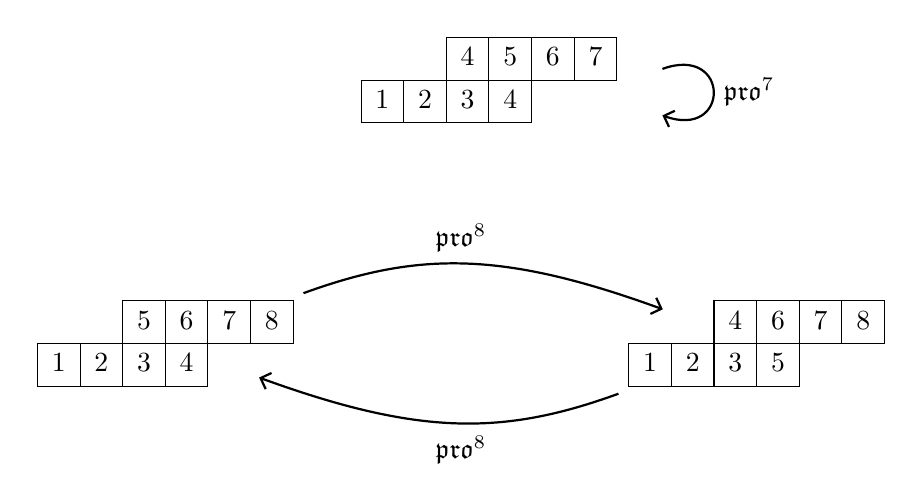
\begin{tikzpicture}
\node (T7) {\ytableaushort{\none \none 4567,1234}};
\node[above right = -0.7 and .2 of T7] (fake1) {};
\node[above right = -1.2 and .2 of T7] (fake2) {};
\node[below left = 2 and 0.6 of T7] (T8A) {\ytableaushort{\none \none 5678,1234}};
\node[right = 4 of T8A] (T8B) {\ytableaushort{\none \none 4678,1235}};
\path (T8A) edge[pil, out=20,in=160,shorten >=-6mm] node[above]{$\pro^8$} (T8B);
\path (T8B) edge[pil, out = 200, in=340,shorten >=-6mm] node[below]{$\pro^8$} (T8A);
\path (fake1) edge[pil, out = 20, in = 340, looseness=4] node[right]{$\pro^7$} (fake2);
\end{tikzpicture}
\caption{The set $\incgl(P_4)$ consists of the three illustrated gapless increasing tableaux. The unique element of $\incgl^7(P_4)$ forms a singleton $\pro^7$-orbit, while $\pro^8$ switches the two elements of $\incgl^8(P_4)$, as shown. The situation for $p \neq 4$ is exactly analogous.}\label{fig:propeller_orbits}
\end{figure}

\begin{table}[h]
\begin{tabular}{|c|c|c|}
\hline
$m_T$ & period ($\tau$) & number of orbits ($N$)\\
  \hline
  $2p-1$ & 1 & 1\\
  \hline
  $2p$ & 2 & 1\\ 
  \hline
\end{tabular}
\caption{The distribution of $\pro^{m_T}$-orbits of gapless increasing tableaux in $\incgl^{m_T}(P_p)$ for each ${m_T}$.}
\label{tab:prop}
\end{table}

 Additionally, we need the fact that the number of elements of $\binom{[i]}{j}$ of any fixed $\Sigma^i$-order is given explicitly by \cite[Theorem~1.1(b)]{Reiner.Stanton.White}:
\begin{theorem}[Reiner, Stanton, and White]\label{thm:rsw}
Let 
\begin{equation*}
f_{i,j}(q) \coloneqq 
\begin{cases}
 \frac{[i]!_q}{[j]!_q\cdot [i-j]!_q} & \text{if } i \geq j \\
 0 & \text{if } i < j 
\end{cases}
\end{equation*}
where $[\ell]!_q \coloneqq \prod_{a=1}^\ell [a]_q$ and $[a]_q \coloneqq \sum_{b = 0}^{a-1} q^b$ are the standard $q$-analogues. Then, 
\[\#\left\{ v \in \binom{[i]}{j} : (\Sigma^i)^{\circ s}(v) = v \right\} = f_{i,j}(\zeta^s),\] where $\zeta$ is any primitive $i$th root of unity. \qed
\end{theorem} 
We will use Theorems~\ref{thm:periodthm} and~\ref{thm:rsw}, together with the data of Tables~\ref{tab:E6},~\ref{tab:E7}, and~\ref{tab:prop}, to completely determine the multiset of $\pro^m$-orbit cardinalities on any set $\inc^m(P)$ for $P \in \{P_p, P_{CM}, P_F \}$. These tables, along with Corollary~\ref{corr:pdbound}, immediately give the period of $\pro^m$.
\\
\begin{theorem}~\label{thm:actualpdbound}
For $m \gg 0$, the period of $\pro^m$ on $\inc^m(P)$ is 
\begin{itemize}
\item $m$ for $P = P_p$, 
\item $m$ for $P = P_{CM}$, and 
\item $3m$ for $P = P_F$. 
\end{itemize}
(Here `$m \gg 0$' means $m \geq 2p$ for $P = P_p$, $m \geq 12$ for $P = P_{CM}$, and $m \geq 22$ for $P = P_F$.) For $m \in \lbrace 18,19,20, 21 \rbrace$, the period of $\pro^m$ on $\inc^m(P_F)$ is $m$.
\end{theorem}
\begin{proof}
Inspecting Table~\ref{tab:E6} shows that, for $P_{CM}$, the period of each gapless tableau  divides its height ($m_T$). By Corollary~\ref{corr:pdbound}, this implies that for any $m$, the $\pro^m$-period of each tableau divides $m$. Clearly the $\pro^{12}$-period of $P_{CM}$ is $12$, and whenever $m> 12$, it is possible to find a tableau attaining period $m$ by taking a gapless tableau $T \in \incgl^{12}(P_{CM})$ with period $12$ and then inflating according to a content vector with $\Sigma^m$-period $m$. The analogous calculation for $P = P_p$ is easy by inspection of Table~\ref{tab:prop}.

The argument is identical for $P = P_F$ when $m \in \lbrace 18,19,20, 21 \rbrace$, but when $m \geq 22$, we do not have that the period of each gapless tableau divides its height. However, inspecting Table~\ref{tab:E7} shows that, for $P_F$, the period of all gapless tableaux of height $q$ divides $3q$ for each $q$. Therefore, Corollary~\ref{corr:pdbound} gives that for every $m$, the period of each tableau divides $3m$. When $m \geq 22$, it is possible to find a tableau attaining period $3m$ by taking a gapless tableau  $T \in \incgl^{22}(P_F)$ with period $66$ and inflating according to a content vector of $\Sigma^m$-period $m$.


\end{proof}


For specified $P \in \{P_p, P_{CM}, P_F\}$, we denote by $m_T\{i\}$, $\tau\{i\}$, and $N\{i\}$ the $i$th element of the first, second, and third columns of the corresponding table, respectively. 
\\

\begin{theorem}~\label{thm:mainresult}
Fix $P \in \lbrace  P_p, P_{CM} \rbrace$, $m \gg 0$, and $d$ dividing $m$. Let $\mathcal{R}(P,m,d)$ be the number of increasing tableaux $T \in \inc^m(P)$ whose $\pro^m$-period divides $m/d$. Then,
\begin{equation}\label{eq:mainresulteq} 
\mathcal{R}(P,m,d)  = \sum \limits_{i: \, d \, \vert \, \frac{m_T\{i\}}{\tau\{i\}}} \tau\{i\} \, N\{i\} \, f_{m,m_T}(\zeta^{m/d}).
\end{equation}
\end{theorem}
\begin{proof}
Theorem~\ref{thm:compressbijective} gives that tableaux of height $m$ correspond bijectively to pairs of gapless tableaux and content vectors of length $m$ with $m_T$ ones, where $m_T$ is the height of the gapless tableau. The table corresponding to $P$ gives all possible gapless tableaux. We loop over the rows of the table and determine for each row how many content vectors yield height-$m$ tableaux whose periods divide $m/d$. 

For each $i$, let $c\{i\} = m_T\{i\}/\tau\{i\}$. By Theorem~\ref{thm:periodthm}, a gapless tableau of height $m_T\{i\}$ and a content vector with period $m\{i\}/d'$ give a tableau of period \[ \frac{\frac{m\{i\}}{d'} \frac{m_T\{i\}}{c\{i\}}}{\gcd(\frac{m_T\{i\}}{d'},\frac{m_T\{i\}}{c\{i\}})} = \frac{\frac{m\{i\}}{d'} \frac{m_T\{i\}}{c\{i\}}}{\frac{m_T\{i\} \, \gcd(c\{i\},d')}{d' c\{i\}}} = \frac{m\{i\}}{\gcd(c\{i\},d')}. \] 
Therefore, the tableau has period dividing $m\{i\}/d$ if and only if $d$ divides both $d'$ and $c\{i\}$. Now $d$ divides $d'$ if and only if the period of the content vector divides $m\{i\}/d$. But the number of content vectors of length $m\{i\}$ with $m_T\{i\}$ ones and with period dividing $m\{i\}/d$ is precisely $f_{m,m_T}(\zeta^{m/d})$ (Theorem~\ref{thm:rsw}).
\end{proof}

The resulting formula is simple enough to check by hand. As in \cite[Proof of Theorem 7.1]{Reiner.Stanton.White}, the following elementary identity allows us to work with integers rather than $q$-integers. 


\begin{lemma}\label{lem:evalq}
Let $\zeta$ be a primitive $N$th root of unity and let $d \divides N$. Then $[n]_{\zeta^{N/d}} = 0$ if and only if $n \equiv 0 \mod d$. Moreover, if $n_1 \equiv n_2 \mod d$, then 
\begin{equation}\label{eq:evalq}
\pushQED{\qed}
\lim \limits_{q \rightarrow \zeta^{N/d}} \frac{[n_1]_q}{[n_2]_q} = 
\begin{cases}
\frac{n_1}{n_2}, &\text{if }  n_1 \equiv n_2 \equiv 0 \mod d; \\
1, &\text{if } n_1 \equiv n_2 \neq 0 \mod d.
\end{cases} \qedhere \popQED
\end{equation}
\end{lemma}

For example, we evaluate $f_{P_p}(\zeta^{m/d})$ for some $d > 1$ dividing both $m$ and $p$. By definition,
\[ f_{P_p}(\zeta^{m/d}) = \frac{[m-(2p-2)]_{\zeta^{m/d}}[m-(2p-2)+1]_{\zeta^{m/d}} \cdots [m-(p-1)]_{\zeta^{m/d}}^2 \cdots [m-1]_{\zeta^{m/d}}[m]_{\zeta^{m/d}}}{[1]_{\zeta^{m/d}}[2]_{\zeta^{m/d}} \cdots [p]_{\zeta^{m/d}}^2 \cdots [2p-2]_{\zeta^{m/d}}[2p-1]_{\zeta^{m/d}}}.\]
Lemma~\ref{lem:evalq} allows us to convert this to a ratio of polynomials by matching equivalence classes modulo $d$ in the numerator and denominator. We see that the numerator and denominator have the same multisets of equivalence classes modulo $d$. Pairing equivalent terms and using the lemma, we have
\[ f_{P_p}(\zeta^{m/d}) = \frac{(m-(2p-d)) \cdots  (m)}{(d) \cdots  (2p-d) p} = \frac{2p}{p}  \binom{m/d}{2p/d} = 2 \binom{m/d}{2p/d}.\]     

An important special case allows us to improve Theorem~\ref{thm:rsw}. We have that for any $i, j \in \mathbb{Z}_{> 0}$, if $\zeta$ is an $i$th root of unity and $d$ divides $\gcd(i,j)$, then
\begin{equation}~\label{eq:evalstraightshape}
f_{i,j}(\zeta^{i/d}) = \binom{i/d}{j/d} = \frac{(i-(j-d))(i-(j-2d)) \cdots  (i-d)(i)}{(d)  (2d)  \cdots  (j-d) (j)}. 
\end{equation}
This equation holds even when $j > i$, since in that case one of terms in the numerator is $0$. 



\begin{proof}[Proof of Theorem~\ref{thm:propeller}] Fix positive integers $p$ and $m$, and suppose $d$ divides $m$. We have that \[ f_{P_p}(\zeta) = \frac{[m]!_q [m-(p-1)]_q}{[2p-1]!_q [m-(2p-1)]!_q [p]_q }.\]  If $d = 1$, then by Theorem~\ref{thm:mainresult}, 
\[ \mathcal{R}(P_p,m,d) = f_{m,2p-1}(1) + 2 \, f_{m,2p}(1) = \binom{m}{2p-1} + 2 \binom{m}{2p} = \frac{(2m-2p+2)m!}{(2p)!(m-2p+1)!} = f_{P_p}(1). \]
Now for $d > 1$, we can have that $d$ divides $p$, or $d$ divides $2p-1$, or $d$ divides neither. If $d$ divides $p$, then by Equation~\ref{eq:evalstraightshape},
\[ \mathcal{R}(P_p,m,d) = 2 \, f_{m,2p}(\zeta^{m/d}) = 2\binom{m/d}{2p/d} = f_{P_p}(\zeta^{m/d}).\]

If $d$ divides $2p-1$,  then
\[ \mathcal{R}(P_p,m,d) =  f_{m,2p-1}(\zeta^{m/d}) = \binom{m/d}{(2p-1)/d} = f_{P_p}(\zeta^{m/d}).\]
If $d$ divides neither $p$ nor $2p-1$, then on the one hand Theorem~\ref{thm:mainresult} predicts that $\mathcal{R}(P_p,m,d) = 0$, and on the other hand $d$ divides $\lceil{\frac{2p-1}{d}}\rceil$ of the terms in the numerator of $f_{P_p}(\zeta^{m/d})$ and at most $\lfloor{\frac{2p-1}{d}}\rfloor$ of the terms in the denominator, so $f_{P_p}(\zeta^{m/d}) = 0$. 
\end{proof}

The verification for $P = P_{CM}$ is similarly straightforward. 

\begin{proof}[Proof of Theorem~\ref{thm:exceptionals}]
Theorem~\ref{thm:F_bad} proves the $P_F$ cases. Hence, it remains to consider $P = P_{CM}$.

Inspecting Table~\ref{tab:E6}, we see that the possible values of $\ell\{i\} = m_T\{i\}/\tau\{i\}$ are $1,11,2,4$ and $8$. Therefore we evaluate $\mathcal{R}(P_{CM},m,d)$ for each $d$ that divides one or more of these $\ell$ values. We verify that this matches the prediction given by $f^m_{CM}$, and that $f^m_{CM}$ predicts $\mathcal{R}(P_{CM},m,d) = 0$ for all $d$ not dividing any of these integers.
\begin{itemize}
\item If $d$ divides $1$, then Theorem~\ref{thm:mainresult} predicts 
\begin{align*}
\mathcal{R}(P_{CM},m,1) &= 1 \cdot 1 \cdot \binom{m}{11} + (3 \cdot 1  + 12 \cdot 1)  \cdot \binom{m}{12} + 13 \cdot 6 \cdot \binom{m}{13} + (7\cdot 2 + 14 \cdot 12) \binom{m}{14}  \\ &\ \ \ \ \ \ + 15 \cdot 13 \cdot \binom{m}{15} + (2 \cdot 1 + 4 \cdot 1 + 8 \cdot 1 + 16 \cdot 4) \binom{m}{16} \\
&= \frac{(m-10)(m-9)(m-8)(m-7)^2(m-6)^2(m-5)^2(m-4)^2(m-3)^2(m-2)(m-1)m}{1\cdot 2\cdot 3\cdot 4^2 \cdot 5^2 \cdot 6^2 \cdot 7^2 \cdot 8^2 \cdot 9 \cdot 10 \cdot 11} \\
&= f_{CM}^m(1).
\end{align*}
\item If $d$ divides $11$ but not $1$, Theorem~\ref{thm:mainresult} predicts
\begin{align*}
\mathcal{R}(P_{CM},m,11) &= 1 \cdot 1 \cdot \binom{m/11}{11/11} \\
&= m/11 \\ 
&= f_{CM}^m(\zeta^{m/11}).
\end{align*}
\item If $d$ divides $8$ but not $4$, Theorem~\ref{thm:mainresult} predicts
\begin{align*}
\mathcal{R}(P_{CM},m,8) &= 2 \cdot 1 \cdot \binom{m/8}{16/8} \\
&= \frac{(m)(m-8)}{8^2} \\
&= f_{CM}^m(\zeta^{m/8}).
\end{align*}
\item If $d$ divides $4$ but not $2$, Theorem~\ref{thm:mainresult} predicts
\begin{align*}
\mathcal{R}(P_{CM},m,4) &= 3 \cdot 1 \cdot \binom{m/4}{12/4} + (4 \cdot 1 + 2 \cdot 1) \cdot \binom{m/4}{16/4}  \\
&= \frac{(m-8)(m-4)^2m}{4^2 \cdot 8^2} \\
&= f_{CM}^m(\zeta^{m/4}).
\end{align*}
\item If $d$ divides $2$ but not $1$, Theorem~\ref{thm:mainresult} predicts
\begin{align*}
\mathcal{R}(P_{CM},m,2) &= 3 \cdot 1 \cdot \binom{m/2}{12/2} + 7 \cdot 2 \cdot \binom{m/2}{14/2} + (2 \cdot 1 + 4 \cdot 1 + 8 \cdot 1) \cdot \binom{m/2}{16/2} \\
&= \frac{(m-10)(m-8)(m-6)^2(m-4)^2(m-2)m}{10 \cdot 8^2 \cdot 6^2 \cdot  4^2 \cdot 2}\\
&= f_{CM}^m(\zeta^{m/2}).
\end{align*}
\end{itemize}
This exhausts all possible $d$ dividing one of the above integers. To see that the cyclic sieving polynomial predicts all other $d$ values are $0$, we first observe that $f^m_{CM}(\zeta^{m/d}) = 0$ if $d > 11$. For in this case, Lemma~\ref{lem:evalq} implies that one of the numerator terms (namely, $[m]_{\zeta^{m/d}}$) is zero, while none of the denominator terms are. 

Using the same identity to count zeros in the numerator and denominator, it is easily checked that the remaining values of $d \leq 11$ evaluate to $0$. 
\end{proof}

\begin{theorem}\label{thm:F_bad}
Conjecture~\ref{conj:rush.shi} holds for $P_F$ only when $k \leq 4$.
\end{theorem}
\begin{proof}
That Conjecture~\ref{conj:rush.shi} holds for $P_F$ in the case $k \leq 4$ can be checked numerically using Table~\ref{tab:E7} and Theorem~\ref{thm:mainresult}.
%note that if you only look at the first 4 rows you don't tend to recover the symbolic expression of the cyclic sieving polynomial, because this requires a lot of terms that are zeroed out at low values.

It remains to show that the conjecture fails for $k \geq 5$. Hence, let $m \geq 22 = 5 +  \rank(P_F) + 1$. By Theorem~\ref{thm:actualpdbound}, $\pro^m$ has order $3m$ on $\inc^m(P_F)$. 

Suppose $T \in \inc^m(P_F)$ were fixed by $\pro^m$.  By Equation~\ref{eq:period}, the $\Sigma^m$-period of $\content^m(T)$ is $1$. Since $\content^m(T)$ is certainly not a vector of all $0$'s, it must therefore be a vector of all $1$'s. Hence, $m_T = m$ and $\deflate(T) = T$. Therefore, $T$ is gapless. However, Table~\ref{tab:E7} shows that no element of $\incgl^m(P_F)$ is fixed by $\pro^m$, for any $m \geq 22$, so such a $T$ does not exist.

%Therefore $\gcd{(m_T/d,\tau)} = 1$, where $\tau$ is the full-content period of the tableau. But then Equation~\ref{eq:period} implies that $\tau = 1$. However, there are no full-content tableau of height $22$ and orbit size $1$. Therefore, there are no tableau fixed by $\pro^{22}$. Theorem~\ref{thm:periodthm} and Table~\ref{tab:E7} allow us to compute that there are $0$ tableaux fixed by $\pro^{22}$.

Now, let $\zeta$ be a primitive $(3m)$th root of unity. By the above, Conjecture~\ref{conj:rush.shi} claims that $f_{P_F}(\zeta) = 0$. But this is impossible, for if $f_{P_F}(\zeta) = 0$, then the minimal polynomial of $\zeta$ would divide the numerator of $f_{P_F}$, which is the product of polynomials of the form $1-q^n$ where $n < 3m$. Thus, Conjecture~\ref{conj:rush.shi} fails in these cases. 
\end{proof}

\section*{Acknowledgements}
The authors thank Julianna Tymoczko for introducing them to each other. OP was partially supported by a Mathematical Sciences Postdoctoral Research Fellowship from the National Science Foundation. HM was supported by the Graduate Research Fellowship from the National Science Foundation. 


%%%%%%%%%%%%%%%%%%%%%%%%%%%%%%%%%%%%%%%%%%%%%%%%%%%%%%%%%%%%
%
%  Bibliography
%
%%%%%%%%%%%%%%%%%%%%%%%%%%%%%%%%%%%%%%%%%%%%%%%%%%%%%%%%%%%%


\bibliographystyle{amsalpha} 
\bibliography{exceptional}



\end{document}
